%--------------------------------------------------------------------------
% Appendix
%--------------------------------------------------------------------------

\appendix

\begin{appendices}

\chapter{Supplementary: Literature Review}
\label{sup: supplementary-litrev}

This Literature Review appendix presents the hierarchical structure of land cover classification adopted for the 2003/2010 NFA in the Philippines.
	\vspace*{10cm}

%\section{Hierarchical structure of land cover classification adopted for the 2003/2010 NFA in the Philippines.}
%\label{app: appendix-hierarch-structure}

\begin{spacing}{1.0}
\begin{longtable}[h!]{ p{6cm} p{8cm} }

    \caption[LCCS hierarchical structure adopted for the 2003/2010 NFA in the Philippines.]{Hierarchical structure of land cover classification adopted for the 2003/2010 NFA in the Philippines (Source: FAO, 2005, 2010).}
    \label{tab: appendix-table.a1}\\
    
    \toprule
    Land cover/forest type & Definition \\
    \midrule
    \endhead

    Closed forest, broadleaved & \multirow{10}{8cm}[1cm]{Land spanning more than 0.5 ha with trees higher than 5 m and a canopy cover of more than 10\%, or trees able to reach these thresholds in situ. It does not include land that is predominantly under agricultural or urban land use.}\\
    Closed forest, coniferous & {}\\
    Closed forest, mixed & {}\\
    Open forest, broadleaved & {}\\
    Open forest, coniferous & {}\\
    Open forest, mixed & {}\\
    Mangrove forest & {}\\
    Forest plantation, broadleaved & {}\\
    Forest plantation, coniferous & {}\\
    Forest plantation, mixed & {}\\[3pt]
    
    \cmidrule{1-2}
    
    Other wooded land, shrubs & \multirow{7}{8cm}[0cm]{Land not classified as \enquote{Forest}, spanning more than 0.5 ha; with trees higher than 5 m and a canopy cover of 5-10\%, or trees able to reach these thresholds in situ; or with a combined cover of shrubs, bushes and trees above 10\%. It does not include land that is predominantly under agricultural or urban land use.}\\
    Other wooded land, fallow & {}\\
    Other wooded land, wooded grassland & {}\\
    {} & {}\\
    {} & {}\\
    {} & {}\\
    {} & {}\\[3pt]
    
    \cmidrule{1-2}
	
	Other land, barren land & \multirow{6}{8cm}[1cm]{All land that is not classified as \enquote{Forest} or \enquote{Other wooded land}.}\\
    Other land, grassland & {}\\
    Other land, marshland & {}\\
    Other land, annual crop & {}\\
    Other land, perennial crop & {}\\
    Other land, built-up area & {}\\[3pt]
    
    \cmidrule{1-2}
    
    Inland water & \multirow{2}{8cm}{Inland water bodies generally include major rivers, lakes and water reservoirs.}\\
    Fishpond & {}\\

	
    \bottomrule
\end{longtable}
\end{spacing}


\chapter{Supplementary: Methods}
\label{sup: supplementary-methods}

This Methods appendix presents the land area statistics of forest cover types per province based on NAMRIA 2010 land cover map, and images of segmentation tests and the selected segmentation parameters.

%\section{NAMRIA 2010 land cover statistics.}
%\label{app: appendix-namria-lc-stats}

\begin{landscape}
\begin{spacing}{1.0}
\begin{longtable}[h!]{ @{}lrrrrrrrrrrrr@{} }
	%{ p{2.5cm} p{1cm} p{1cm} p{1cm} p{1cm} p{1cm} p{1cm} p{1cm} p{1cm} p{1cm} p{2cm} p{2cm} }

    \caption[Land area statistics of forest cover types per province based on NAMRIA 2010 land cover map.]{Land area statistics of forest cover types per province based on NAMRIA 2010 land cover map.}
    \label{tab: appendix-table.b1}\\
    
    	\toprule
    	Province & FCFB & FCFC & FCFM & FOFB & FOFC & FOFM & FFPB & FFPC & LVMG & NF & Total (ha)\\ 
    	\midrule
    	\endhead
    	
    	Abra & 27,025 & 9,812 & 6,479 & 54,884 & 35,508 & 11,119 & 1,874 & {} & {} & 250,940 & 397,640\\
    	Apayao & 95,704 & {} & {} & 17,353 & {} & {} & 10,023 & {} & {} & 59,469 & 182,549\\
    	Aurora & 51,933 & {} & {} & 60,265 & {} & {} & {} & {} & 511 & 49,888 & 162,598\\
    	Benguet & 122 & 3,023 & 51 & 12,055 & 75,580 & 28,786 & {} & 8 & {} & 135,870 & 255,495\\
    	Cagayan & 160,433 & {} & {} & 89,908 & {} & {} & 4,459 & {} & {} & 295,973 & 550,772\\
    	Ifugao & 12,170 & 671 & 851 & 84,327 & 4,379 & {} & {} & {} & {} & 163,577 & 265,974\\
    	Ilocos Norte & 884 & {} & {} & 17,003 & {} & {} & {} & {} & {} & 83,313 & 101,199\\
    	Ilocos Sur & {} & 25 & 53 & 20,270 & 1,229 & 7,277 & 2,154 & 793 & 211 & 239,236 & 271,248\\
    	Isabela & 69,444 & {} & {} & 307,852 & {} & {} & 254 & {} & 723 & 662,263 & 1,040,536\\
    	Kalinga & 40,305 & 22 & 8,561 & 39,113 & 8,949 & 1,912 & {} & {} & {} & 186,971 & 285,833\\
    	La Union & {} & {} & {} & 2,558 & {} & 2,165 & 1,037 & {} & 120 & 139,801 & 145,681\\
    	Mt Province & 17,955 & {} & 9,523 & 20,072 & 32,211 & 7,505 & {} & {} & {} & 110,635 & 197,900\\
    	N. Ecija & 4,310 & {} & {} & 11,824 & {} & 567 & {} & {} & {} & 44,038 & 60,739\\
    	N. Vizcaya & 119,583 & 2,351 & 555 & 57,812 & 5,028 & 5,994 & 1,307 & {}& 217,853 & 410,482\\
    	Pangasinan & 181 & {} & {} & 5,160 & 924 & 280 & 812 & {} & 556 & 304,127 & 312,040\\
    	Quirino & 85,630 & {} & {} & 40,728 & {} & {} & 147 & {} & {} & 141,634 & 268,139\\
    	\cmidrule{1-12}
    	TOTAL & 685,677 & 15,905 & 26,072 & 841,185 & 163,806 & 65,604 & 22,067 & 802 & 2,122 & 3,085,588 & 4,908,827\\
    	\% & 13.97 & 0.32 & 0.53 & 17.14 & 3.34 & 1.34 & 0.45 & 0.02 & 0.04 & 62.86 & 100.00\\
    	\bottomrule
    
\end{longtable}

	\noindent Note: FCFB: Closed forest, broadleaved; FCFC: Closed forest, coniferous; FCFM: Closed forest, mixed; FOFB: Open forest, broadleaved;  FOFC: Open forest, coniferous; FOFM: Open forest, mixed; FFPB: Forest plantation, broadleaved; FFPC: Forest plantation, coniferous; LVMG: Mangrove forest; NF: Non-Forest\\ \newline
	
\end{spacing}
\end{landscape}

%\section{Image segmentation tests.}
%\label{app: appendix-segment-tests}

\begin{figure}
	\centering
	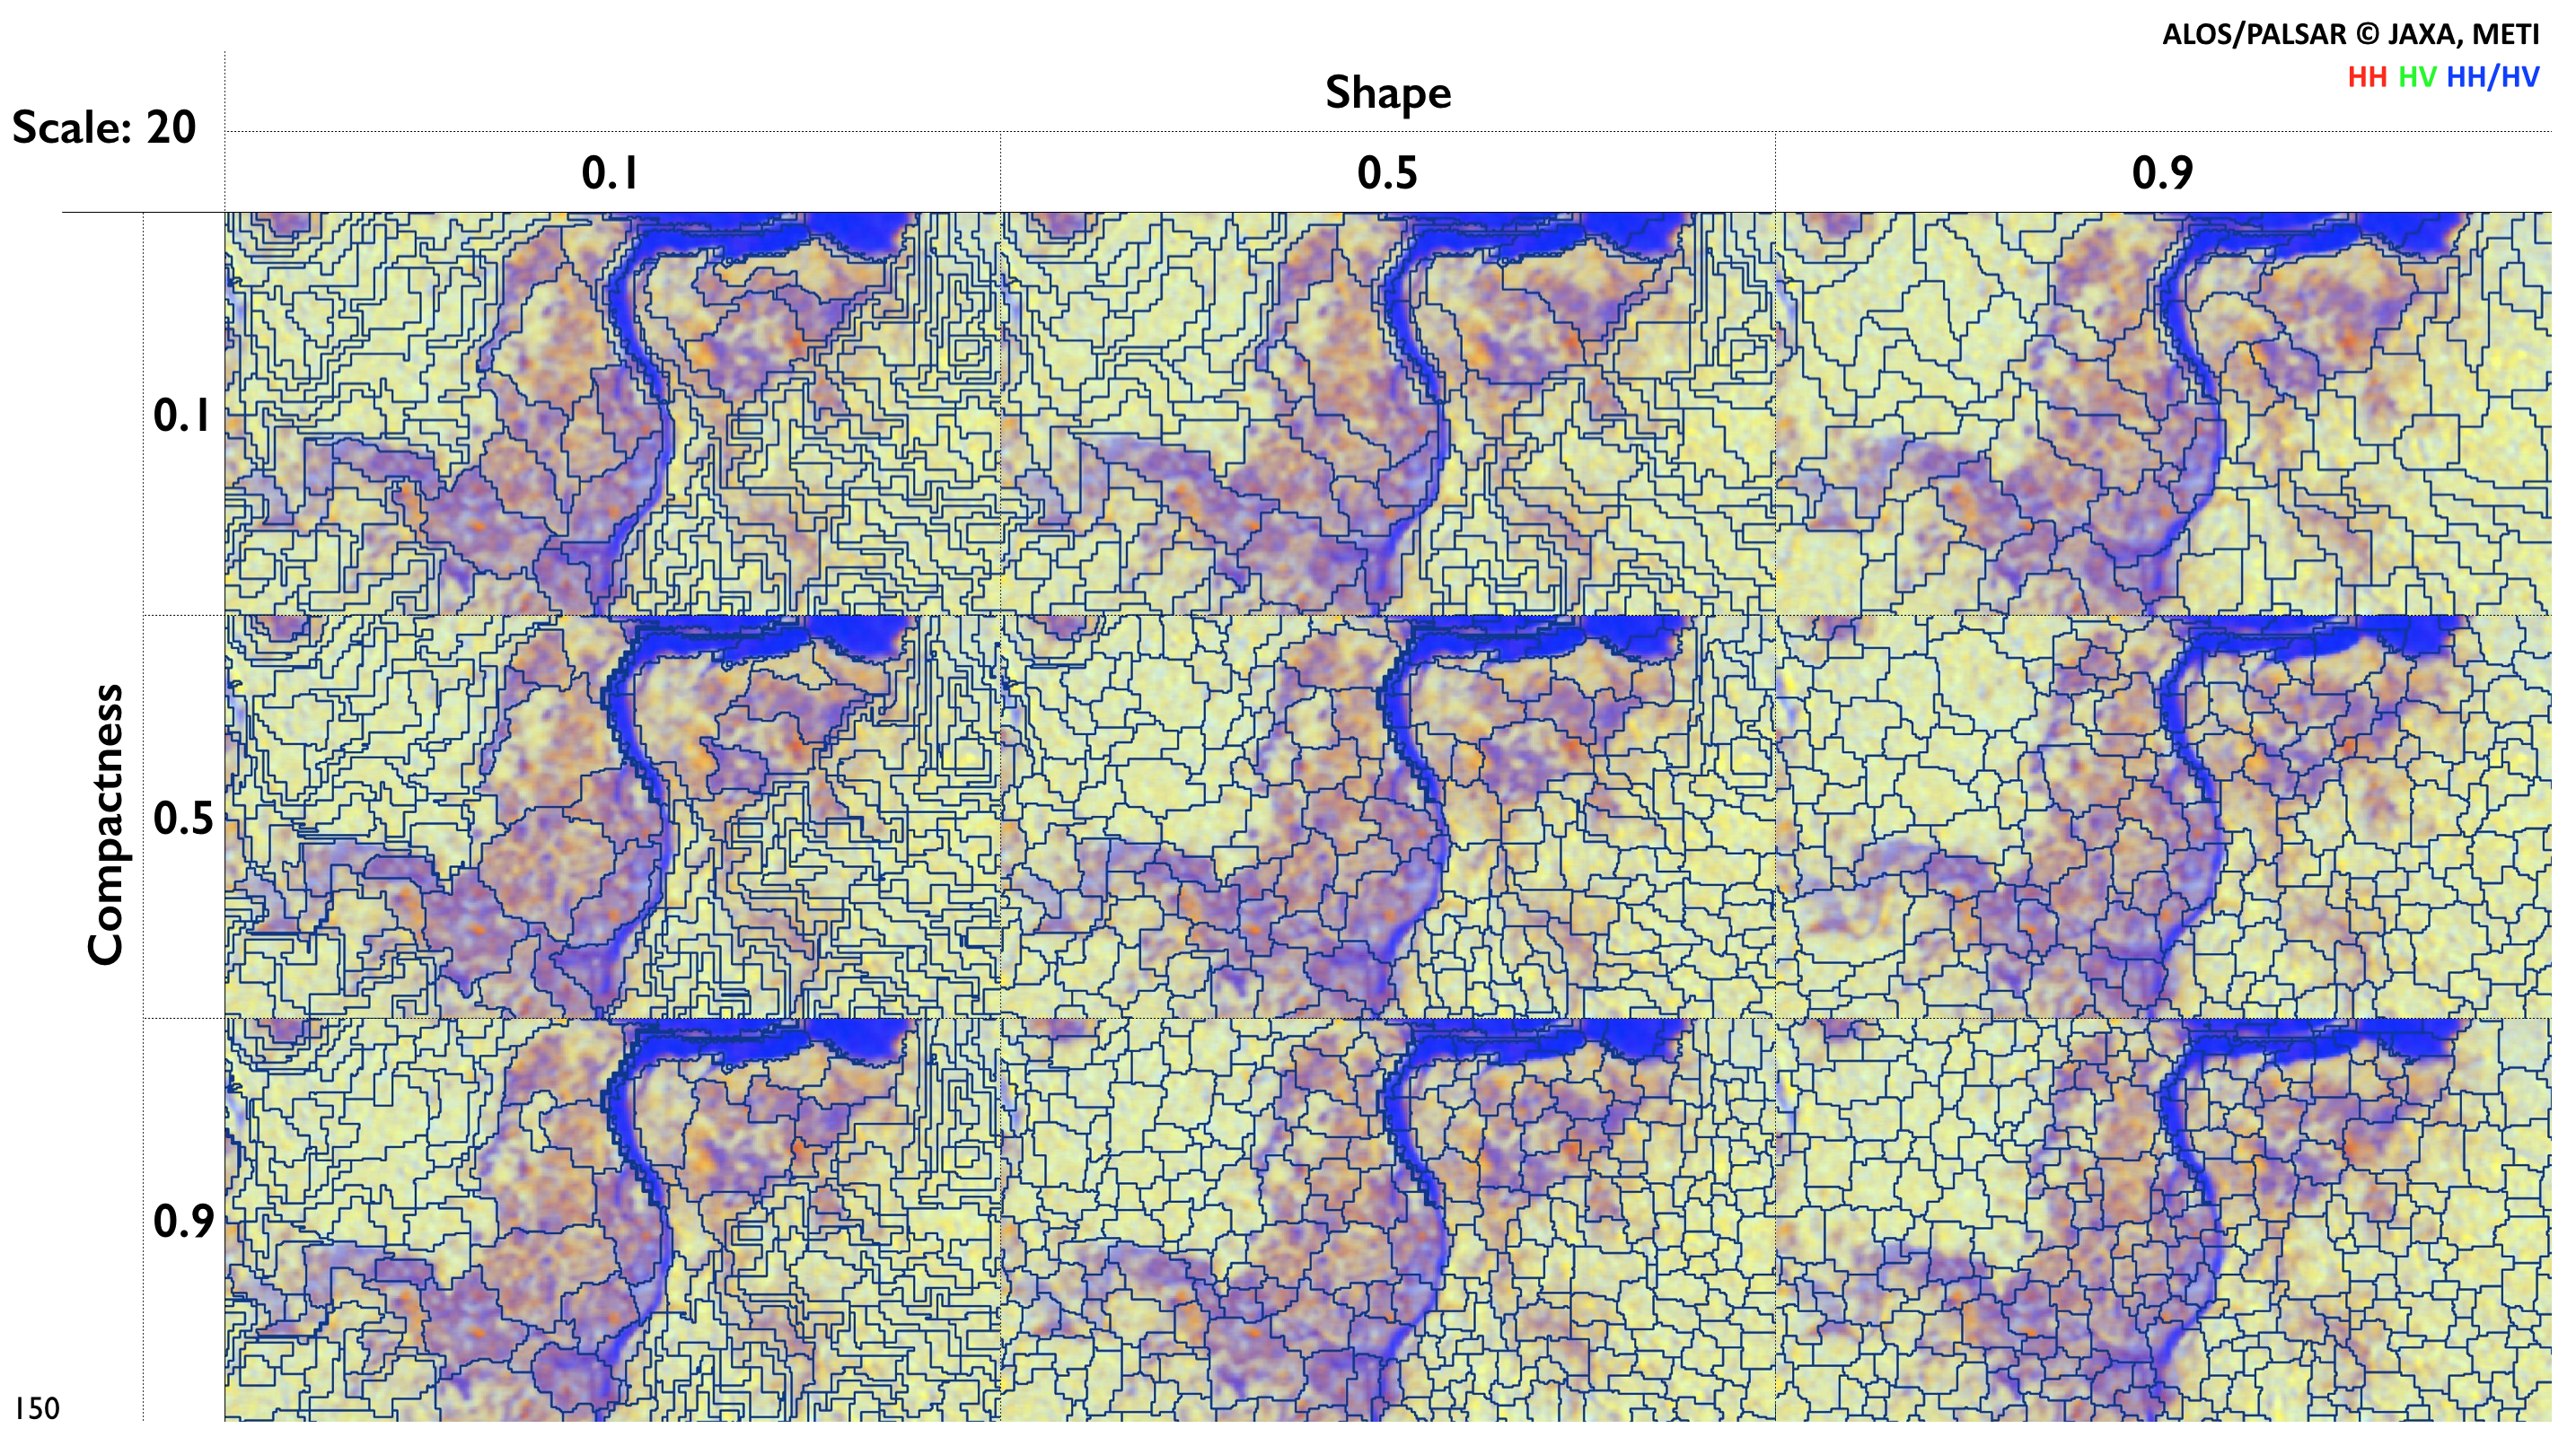
\includegraphics[width=0.9\textwidth]{fig_segmentation-tests.png}
	\caption[Images of segmentation tests.]{Test segmentation images using a scale value of 20 with shape and compactness values set at 0.1, 0.5, and 0.9. Image weights set at 1 for radar and topographic data layers.}
	\label{fig: appendix-fig.b1}
\end{figure}

\begin{figure}
	\centering
	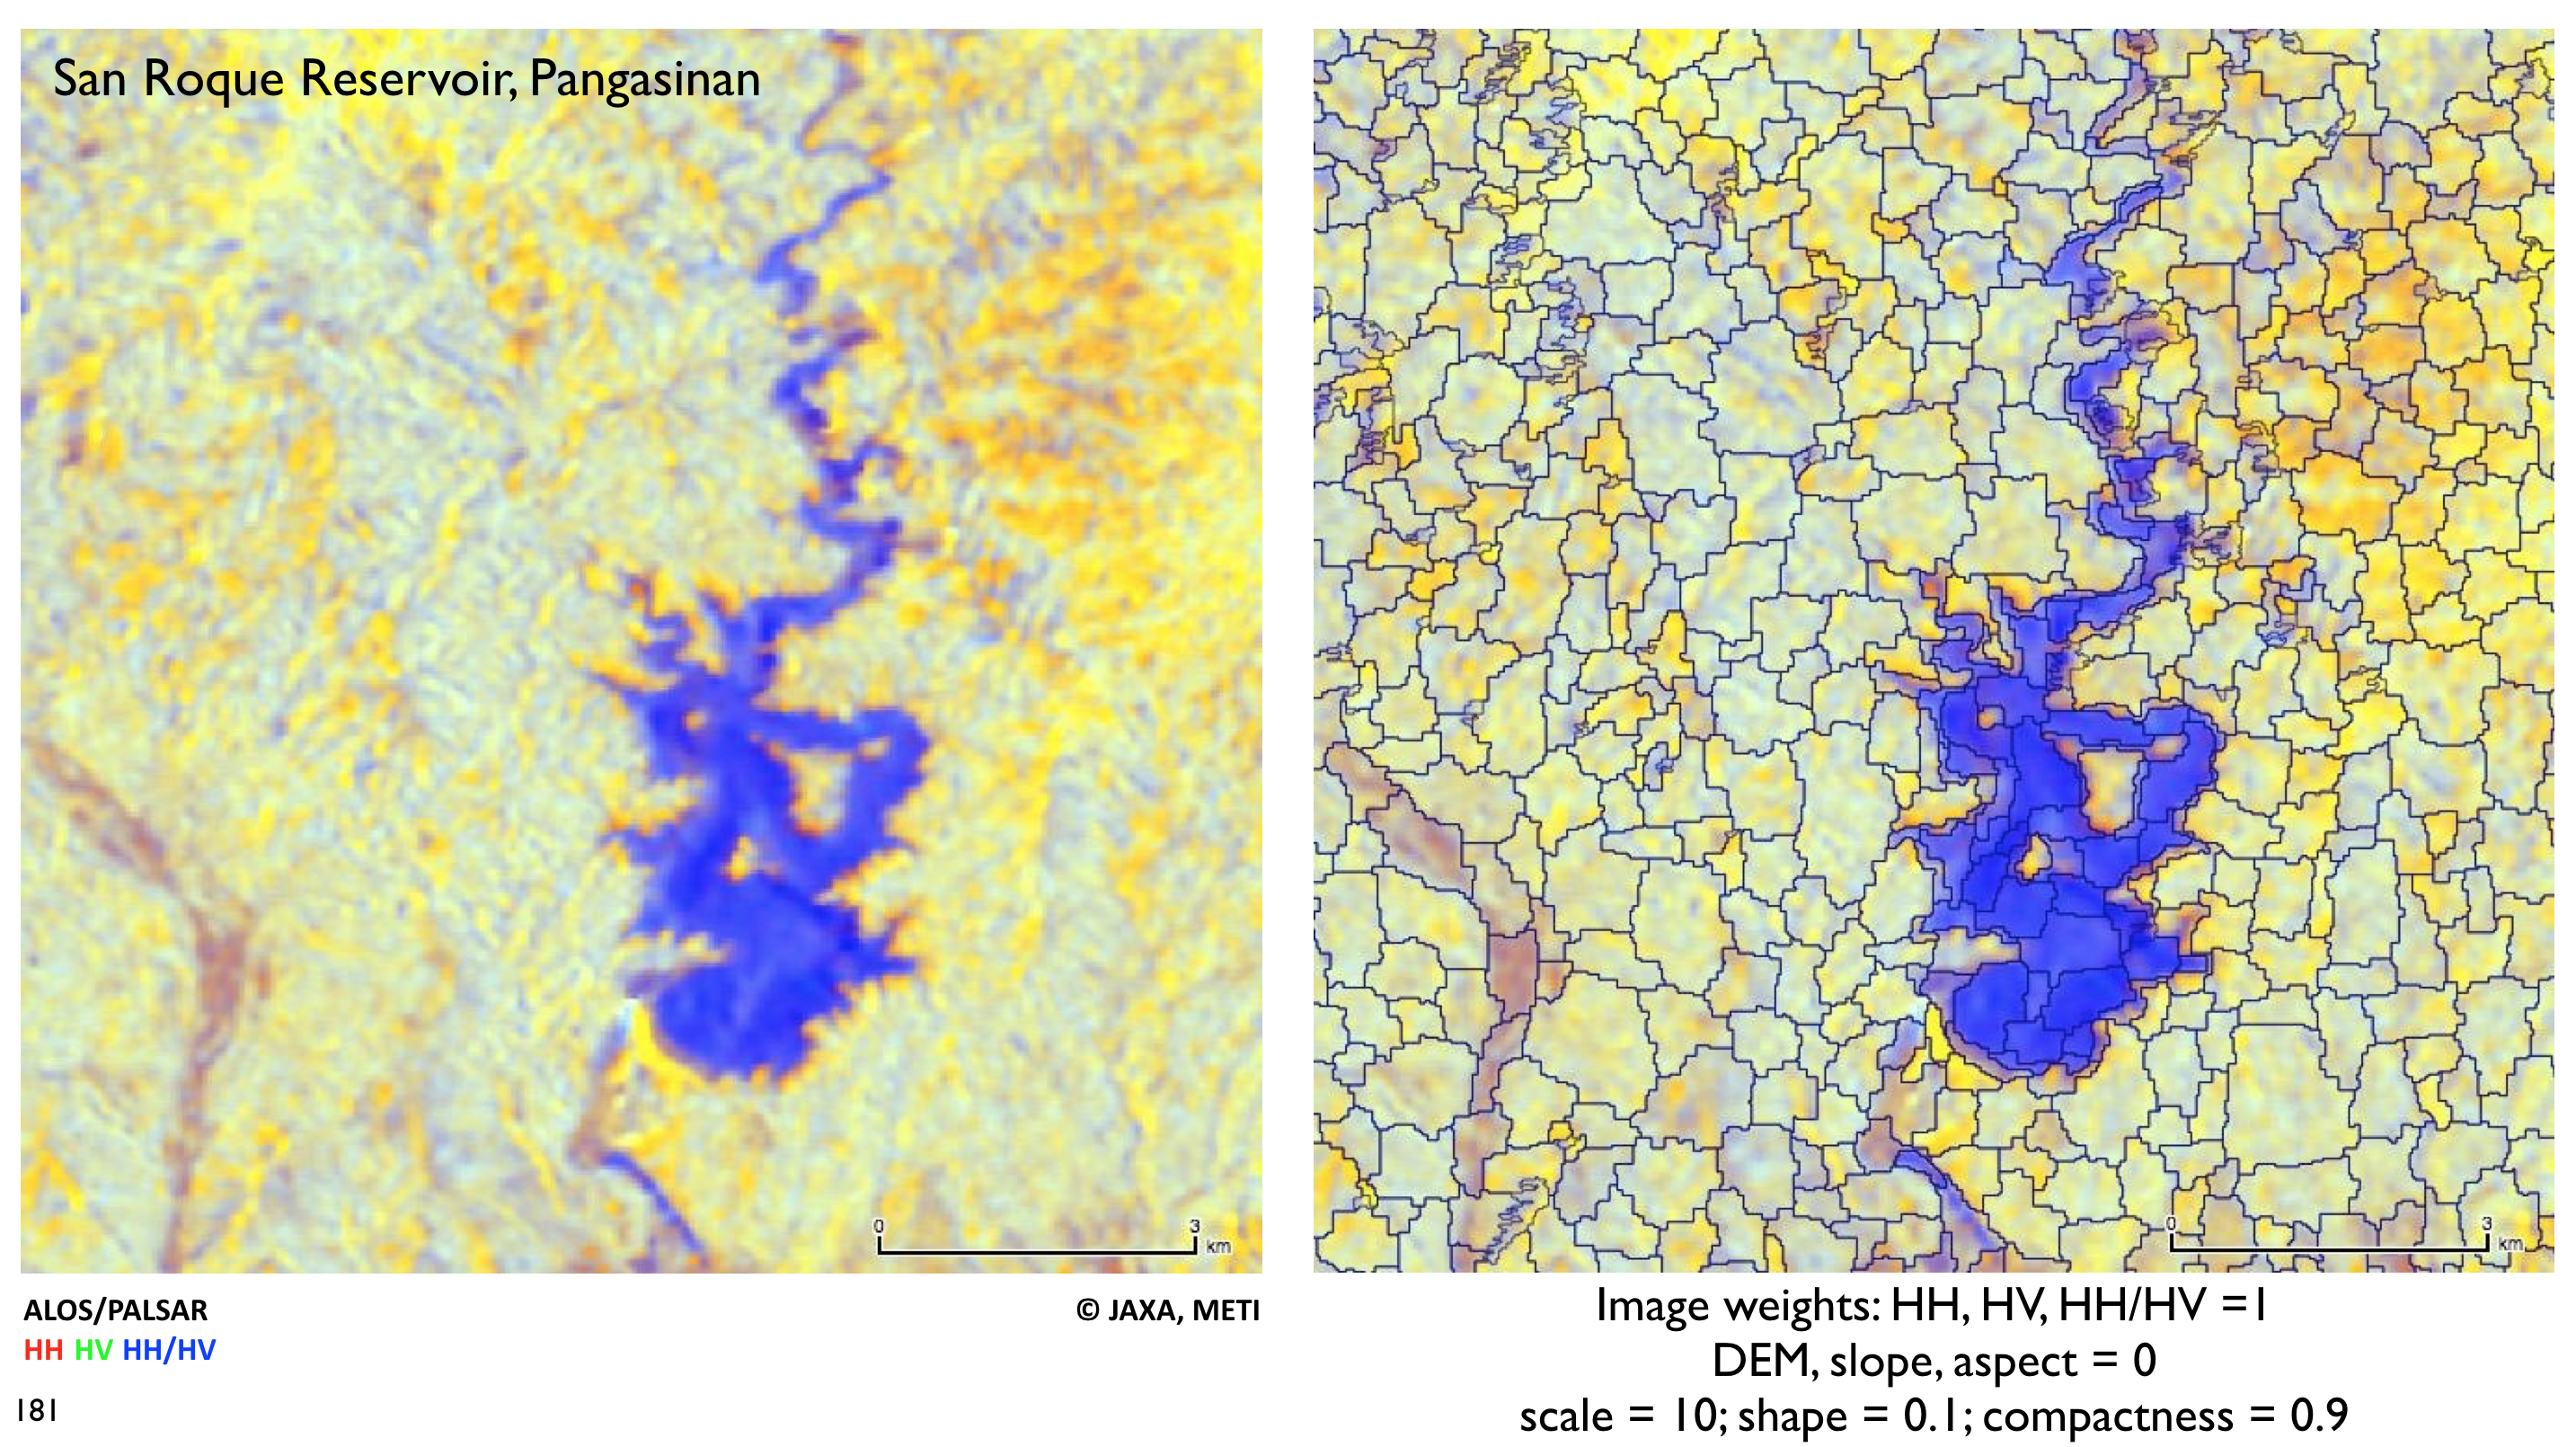
\includegraphics[width=0.9\textwidth]{fig_segmentation-final.png}
	\caption[Images of selected segmentation parameters.]{Selected segmentation parameters using a scale value of 10, shape value of 0.1, and compactness value at 0.9. Image weights set at 1 for radar data layers and 0 for topographic data layers.}
	\label{fig: appendix-fig.b2}
\end{figure}

\chapter{Supplementary: Results}
\label{sup: supplementary-results}

This Results appendix presents the classification trees and cross-validation graphs generated by R tree package.

\section{Classification trees and cross-validation graphs}
\label{app: appendix-trees-graphs}

% CASE 1 2007

\begin{figure}[!ht] \centering
	\captionsetup[subfigure]{width=2.0in}
	\begin{subfigure}[t]{0.32\textwidth}
		\includegraphics[width=\textwidth]{case1-2007-pruned-dendrogram-lc1.pdf}
		\caption{Level 1}
	\end{subfigure}
	\begin{subfigure}[t]{0.32\textwidth}
		\includegraphics[width=\textwidth]{case1-2007-pruned-dendrogram-lc2.pdf}
		\caption{Level 2}
	\end{subfigure}
	\begin{subfigure}[t]{0.32\textwidth}
		\includegraphics[width=\textwidth]{case1-2007-pruned-dendrogram-lc3.pdf}
		\caption{Level 3}
	\end{subfigure}\\
	\vspace{5pt}
	\begin{subfigure}[t]{0.32\textwidth}
		\includegraphics[width=\textwidth]{case1-2007-pruned-dendrogram-lc4.pdf}
		\caption{Level 4}
	\end{subfigure}
	\begin{subfigure}[t]{0.32\textwidth}
		\includegraphics[width=\textwidth]{case1-2007-pruned-dendrogram-lc5.pdf}
		\caption{Level 5}
	\end{subfigure}
	\begin{subfigure}[t]{0.32\textwidth}
		\includegraphics[width=\textwidth]{case1-2007-pruned-dendrogram-lc6.pdf}
		\caption{Level 6}
	\end{subfigure}\\
	\vspace{5pt}	
	\begin{subfigure}[t]{0.32\textwidth}
		\includegraphics[width=\textwidth]{case1-2007-pruned-dendrogram-lc7.pdf}
		\caption{Level 7}
	\end{subfigure}
	\begin{subfigure}[t]{0.32\textwidth}
		\includegraphics[width=\textwidth]{case1-2007-pruned-dendrogram-lc8.pdf}
		\caption{Level 8}
	\end{subfigure}
	\begin{subfigure}[t]{0.32\textwidth}
		\includegraphics[width=\textwidth]{case1-2007-pruned-dendrogram-lc9.pdf}
		\caption{Level 9}
	\end{subfigure}\\
	\vspace{5pt}
	\begin{subfigure}[t]{0.32\textwidth}
		\includegraphics[width=\textwidth]{case1-2007-pruned-dendrogram-lc10.pdf}
		\caption{Level 10}
	\end{subfigure}
	\begin{subfigure}[t]{0.32\textwidth}
		\includegraphics[width=\textwidth]{case1-2007-pruned-dendrogram-lc11.pdf}
		\caption{Level 11}
	\end{subfigure}
	\vspace{5pt}
	\caption[The Case 1 2007 classification trees generated by R tree package.]{The Case 1 2007 classification trees generated by R tree package.}
	\label{fig: appendix-fig.c1.tree}
\end{figure}

\begin{figure}[!ht] \centering
	\captionsetup[subfigure]{width=2.0in}
	\begin{subfigure}[t]{0.32\textwidth}
		\includegraphics[width=\textwidth]{case1-2007-cv-lc1.pdf}
		\caption{Level 1}
	\end{subfigure}
	\begin{subfigure}[t]{0.32\textwidth}
		\includegraphics[width=\textwidth]{case1-2007-cv-lc2.pdf}
		\caption{Level 2}
	\end{subfigure}
	\begin{subfigure}[t]{0.32\textwidth}
		\includegraphics[width=\textwidth]{case1-2007-cv-lc3.pdf}
		\caption{Level 3}
	\end{subfigure}\\
	\vspace{5pt}
	\begin{subfigure}[t]{0.32\textwidth}
		\includegraphics[width=\textwidth]{case1-2007-cv-lc4.pdf}
		\caption{Level 4}
	\end{subfigure}
	\begin{subfigure}[t]{0.32\textwidth}
		\includegraphics[width=\textwidth]{case1-2007-cv-lc5.pdf}
		\caption{Level 5}
	\end{subfigure}
	\begin{subfigure}[t]{0.32\textwidth}
		\includegraphics[width=\textwidth]{case1-2007-cv-lc6.pdf}
		\caption{Level 6}
	\end{subfigure}\\
	\vspace{5pt}	
	\begin{subfigure}[t]{0.32\textwidth}
		\includegraphics[width=\textwidth]{case1-2007-cv-lc7.pdf}
		\caption{Level 7}
	\end{subfigure}
	\begin{subfigure}[t]{0.32\textwidth}
		\includegraphics[width=\textwidth]{case1-2007-cv-lc8.pdf}
		\caption{Level 8}
	\end{subfigure}
	\begin{subfigure}[t]{0.32\textwidth}
		\includegraphics[width=\textwidth]{case1-2007-cv-lc9.pdf}
		\caption{Level 9}
	\end{subfigure}\\
	\vspace{5pt}
	\begin{subfigure}[t]{0.32\textwidth}
		\includegraphics[width=\textwidth]{case1-2007-cv-lc10.pdf}
		\caption{Level 10}
	\end{subfigure}
	\begin{subfigure}[t]{0.32\textwidth}
		\includegraphics[width=\textwidth]{case1-2007-cv-lc11.pdf}
		\caption{Level 11}
	\end{subfigure}
	\vspace{5pt}
	\caption[The Case 1 2007 cross-validation graphs generated by R tree package.]{The Case 1 2007 cross-validation graphs generated by R tree package.}
	\label{fig: appendix-fig.c2.cv}
\end{figure}

% CASE 1 2008

\begin{figure}[!ht] \centering
	\captionsetup[subfigure]{width=2.0in}
	\begin{subfigure}[t]{0.32\textwidth}
		\includegraphics[width=\textwidth]{case1-2008-pruned-dendrogram-lc1.pdf}
		\caption{Level 1}
	\end{subfigure}
	\begin{subfigure}[t]{0.32\textwidth}
		\includegraphics[width=\textwidth]{case1-2008-pruned-dendrogram-lc2.pdf}
		\caption{Level 2}
	\end{subfigure}
	\begin{subfigure}[t]{0.32\textwidth}
		\includegraphics[width=\textwidth]{case1-2008-pruned-dendrogram-lc3.pdf}
		\caption{Level 3}
	\end{subfigure}\\
	\vspace{5pt}
	\begin{subfigure}[t]{0.32\textwidth}
		\includegraphics[width=\textwidth]{case1-2008-pruned-dendrogram-lc4.pdf}
		\caption{Level 4}
	\end{subfigure}
	\begin{subfigure}[t]{0.32\textwidth}
		\includegraphics[width=\textwidth]{case1-2008-pruned-dendrogram-lc5.pdf}
		\caption{Level 5}
	\end{subfigure}
	\begin{subfigure}[t]{0.32\textwidth}
		\includegraphics[width=\textwidth]{case1-2008-pruned-dendrogram-lc6.pdf}
		\caption{Level 6}
	\end{subfigure}\\
	\vspace{5pt}	
	\begin{subfigure}[t]{0.32\textwidth}
		\includegraphics[width=\textwidth]{case1-2008-pruned-dendrogram-lc7.pdf}
		\caption{Level 7}
	\end{subfigure}
	\begin{subfigure}[t]{0.32\textwidth}
		\includegraphics[width=\textwidth]{case1-2008-pruned-dendrogram-lc8.pdf}
		\caption{Level 8}
	\end{subfigure}
	\begin{subfigure}[t]{0.32\textwidth}
		\includegraphics[width=\textwidth]{case1-2008-pruned-dendrogram-lc9.pdf}
		\caption{Level 9}
	\end{subfigure}\\
	\vspace{5pt}
	\begin{subfigure}[t]{0.32\textwidth}
		\includegraphics[width=\textwidth]{case1-2008-pruned-dendrogram-lc10.pdf}
		\caption{Level 10}
	\end{subfigure}
	\begin{subfigure}[t]{0.32\textwidth}
		\includegraphics[width=\textwidth]{case1-2008-pruned-dendrogram-lc11.pdf}
		\caption{Level 11}
	\end{subfigure}
	\vspace{5pt}
	\caption[The Case 1 2008 classification trees generated by R tree package.]{The Case 1 2008 classification trees generated by R tree package.}
	\label{fig: appendix-fig.c3.tree}
\end{figure}

\begin{figure}[!ht] \centering
	\captionsetup[subfigure]{width=2.0in}
	\begin{subfigure}[t]{0.32\textwidth}
		\includegraphics[width=\textwidth]{case1-2008-cv-lc1.pdf}
		\caption{Level 1}
	\end{subfigure}
	\begin{subfigure}[t]{0.32\textwidth}
		\includegraphics[width=\textwidth]{case1-2008-cv-lc2.pdf}
		\caption{Level 2}
	\end{subfigure}
	\begin{subfigure}[t]{0.32\textwidth}
		\includegraphics[width=\textwidth]{case1-2008-cv-lc3.pdf}
		\caption{Level 3}
	\end{subfigure}\\
	\vspace{5pt}
	\begin{subfigure}[t]{0.32\textwidth}
		\includegraphics[width=\textwidth]{case1-2008-cv-lc4.pdf}
		\caption{Level 4}
	\end{subfigure}
	\begin{subfigure}[t]{0.32\textwidth}
		\includegraphics[width=\textwidth]{case1-2008-cv-lc5.pdf}
		\caption{Level 5}
	\end{subfigure}
	\begin{subfigure}[t]{0.32\textwidth}
		\includegraphics[width=\textwidth]{case1-2008-cv-lc6.pdf}
		\caption{Level 6}
	\end{subfigure}\\
	\vspace{5pt}	
	\begin{subfigure}[t]{0.32\textwidth}
		\includegraphics[width=\textwidth]{case1-2008-cv-lc7.pdf}
		\caption{Level 7}
	\end{subfigure}
	\begin{subfigure}[t]{0.32\textwidth}
		\includegraphics[width=\textwidth]{case1-2008-cv-lc8.pdf}
		\caption{Level 8}
	\end{subfigure}
	\begin{subfigure}[t]{0.32\textwidth}
		\includegraphics[width=\textwidth]{case1-2008-cv-lc9.pdf}
		\caption{Level 9}
	\end{subfigure}\\
	\vspace{5pt}
	\begin{subfigure}[t]{0.32\textwidth}
		\includegraphics[width=\textwidth]{case1-2008-cv-lc10.pdf}
		\caption{Level 10}
	\end{subfigure}
	\begin{subfigure}[t]{0.32\textwidth}
		\includegraphics[width=\textwidth]{case1-2008-cv-lc11.pdf}
		\caption{Level 11}
	\end{subfigure}
	\vspace{5pt}
	\caption[The Case 1 2008 cross-validation graphs generated by R tree package.]{The Case 1 2008 cross-validation graphs generated by R tree package.}
	\label{fig: appendix-fig.c4.cv}
\end{figure}

% CASE 1 2009

\begin{figure}[!ht] \centering
	\captionsetup[subfigure]{width=2.0in}
	\begin{subfigure}[t]{0.32\textwidth}
		\includegraphics[width=\textwidth]{case1-2009-pruned-dendrogram-lc1.pdf}
		\caption{Level 1}
	\end{subfigure}
	\begin{subfigure}[t]{0.32\textwidth}
		\includegraphics[width=\textwidth]{case1-2009-pruned-dendrogram-lc2.pdf}
		\caption{Level 2}
	\end{subfigure}
	\begin{subfigure}[t]{0.32\textwidth}
		\includegraphics[width=\textwidth]{case1-2009-pruned-dendrogram-lc3.pdf}
		\caption{Level 3}
	\end{subfigure}\\
	\vspace{5pt}
	\begin{subfigure}[t]{0.32\textwidth}
		\includegraphics[width=\textwidth]{case1-2009-pruned-dendrogram-lc4.pdf}
		\caption{Level 4}
	\end{subfigure}
	\begin{subfigure}[t]{0.32\textwidth}
		\includegraphics[width=\textwidth]{case1-2009-pruned-dendrogram-lc5.pdf}
		\caption{Level 5}
	\end{subfigure}
	\begin{subfigure}[t]{0.32\textwidth}
		\includegraphics[width=\textwidth]{case1-2009-pruned-dendrogram-lc6.pdf}
		\caption{Level 6}
	\end{subfigure}\\
	\vspace{5pt}	
	\begin{subfigure}[t]{0.32\textwidth}
		\includegraphics[width=\textwidth]{case1-2009-pruned-dendrogram-lc7.pdf}
		\caption{Level 7}
	\end{subfigure}
	\begin{subfigure}[t]{0.32\textwidth}
		\includegraphics[width=\textwidth]{case1-2009-pruned-dendrogram-lc8.pdf}
		\caption{Level 8}
	\end{subfigure}
	\begin{subfigure}[t]{0.32\textwidth}
		\includegraphics[width=\textwidth]{case1-2009-pruned-dendrogram-lc9.pdf}
		\caption{Level 9}
	\end{subfigure}\\
	\vspace{5pt}
	\begin{subfigure}[t]{0.32\textwidth}
		\includegraphics[width=\textwidth]{case1-2009-pruned-dendrogram-lc10.pdf}
		\caption{Level 10}
	\end{subfigure}
	\begin{subfigure}[t]{0.32\textwidth}
		\includegraphics[width=\textwidth]{case1-2009-pruned-dendrogram-lc11.pdf}
		\caption{Level 11}
	\end{subfigure}
	\vspace{5pt}
	\caption[The Case 1 2009 classification trees generated by R tree package.]{The Case 1 2009 classification trees generated by R tree package.}
	\label{fig: appendix-fig.c5.tree}
\end{figure}

\begin{figure}[!ht] \centering
	\captionsetup[subfigure]{width=2.0in}
	\begin{subfigure}[t]{0.32\textwidth}
		\includegraphics[width=\textwidth]{case1-2009-cv-lc1.pdf}
		\caption{Level 1}
	\end{subfigure}
	\begin{subfigure}[t]{0.32\textwidth}
		\includegraphics[width=\textwidth]{case1-2009-cv-lc2.pdf}
		\caption{Level 2}
	\end{subfigure}
	\begin{subfigure}[t]{0.32\textwidth}
		\includegraphics[width=\textwidth]{case1-2009-cv-lc3.pdf}
		\caption{Level 3}
	\end{subfigure}\\
	\vspace{5pt}
	\begin{subfigure}[t]{0.32\textwidth}
		\includegraphics[width=\textwidth]{case1-2009-cv-lc4.pdf}
		\caption{Level 4}
	\end{subfigure}
	\begin{subfigure}[t]{0.32\textwidth}
		\includegraphics[width=\textwidth]{case1-2009-cv-lc5.pdf}
		\caption{Level 5}
	\end{subfigure}
	\begin{subfigure}[t]{0.32\textwidth}
		\includegraphics[width=\textwidth]{case1-2009-cv-lc6.pdf}
		\caption{Level 6}
	\end{subfigure}\\
	\vspace{5pt}	
	\begin{subfigure}[t]{0.32\textwidth}
		\includegraphics[width=\textwidth]{case1-2009-cv-lc7.pdf}
		\caption{Level 7}
	\end{subfigure}
	\begin{subfigure}[t]{0.32\textwidth}
		\includegraphics[width=\textwidth]{case1-2009-cv-lc8.pdf}
		\caption{Level 8}
	\end{subfigure}
	\begin{subfigure}[t]{0.32\textwidth}
		\includegraphics[width=\textwidth]{case1-2009-cv-lc9.pdf}
		\caption{Level 9}
	\end{subfigure}\\
	\vspace{5pt}
	\begin{subfigure}[t]{0.32\textwidth}
		\includegraphics[width=\textwidth]{case1-2009-cv-lc10.pdf}
		\caption{Level 10}
	\end{subfigure}
	\begin{subfigure}[t]{0.32\textwidth}
		\includegraphics[width=\textwidth]{case1-2009-cv-lc11.pdf}
		\caption{Level 11}
	\end{subfigure}
	\vspace{5pt}
	\caption[The Case 1 2009 cross-validation graphs generated by R tree package.]{The Case 1 2009 cross-validation graphs generated by R tree package.}
	\label{fig: appendix-fig.c6.cv}
\end{figure}

% CASE 1 2010

\begin{figure}[!ht] \centering
	\captionsetup[subfigure]{width=2.0in}
	\begin{subfigure}[t]{0.32\textwidth}
		\includegraphics[width=\textwidth]{case1-2010-pruned-dendrogram-lc1.pdf}
		\caption{Level 1}
	\end{subfigure}
	\begin{subfigure}[t]{0.32\textwidth}
		\includegraphics[width=\textwidth]{case1-2010-pruned-dendrogram-lc2.pdf}
		\caption{Level 2}
	\end{subfigure}
	\begin{subfigure}[t]{0.32\textwidth}
		\includegraphics[width=\textwidth]{case1-2010-pruned-dendrogram-lc3.pdf}
		\caption{Level 3}
	\end{subfigure}\\
	\vspace{5pt}
	\begin{subfigure}[t]{0.32\textwidth}
		\includegraphics[width=\textwidth]{case1-2010-pruned-dendrogram-lc4.pdf}
		\caption{Level 4}
	\end{subfigure}
	\begin{subfigure}[t]{0.32\textwidth}
		\includegraphics[width=\textwidth]{case1-2010-pruned-dendrogram-lc5.pdf}
		\caption{Level 5}
	\end{subfigure}
	\begin{subfigure}[t]{0.32\textwidth}
		\includegraphics[width=\textwidth]{case1-2010-pruned-dendrogram-lc6.pdf}
		\caption{Level 6}
	\end{subfigure}\\
	\vspace{5pt}	
	\begin{subfigure}[t]{0.32\textwidth}
		\includegraphics[width=\textwidth]{case1-2010-pruned-dendrogram-lc7.pdf}
		\caption{Level 7}
	\end{subfigure}
	\begin{subfigure}[t]{0.32\textwidth}
		\includegraphics[width=\textwidth]{case1-2010-pruned-dendrogram-lc8.pdf}
		\caption{Level 8}
	\end{subfigure}
	\begin{subfigure}[t]{0.32\textwidth}
		\includegraphics[width=\textwidth]{case1-2010-pruned-dendrogram-lc9.pdf}
		\caption{Level 9}
	\end{subfigure}\\
	\vspace{5pt}
	\begin{subfigure}[t]{0.32\textwidth}
		\includegraphics[width=\textwidth]{case1-2010-pruned-dendrogram-lc10.pdf}
		\caption{Level 10}
	\end{subfigure}
	\begin{subfigure}[t]{0.32\textwidth}
		\includegraphics[width=\textwidth]{case1-2010-pruned-dendrogram-lc11.pdf}
		\caption{Level 11}
	\end{subfigure}
	\vspace{5pt}
	\caption[The Case 1 2010 classification trees generated by R tree package.]{The Case 1 2010 classification trees generated by R tree package.}
	\label{fig: appendix-fig.c7.tree}
\end{figure}

\begin{figure}[!ht] \centering
	\captionsetup[subfigure]{width=2.0in}
	\begin{subfigure}[t]{0.32\textwidth}
		\includegraphics[width=\textwidth]{case1-2010-cv-lc1.pdf}
		\caption{Level 1}
	\end{subfigure}
	\begin{subfigure}[t]{0.32\textwidth}
		\includegraphics[width=\textwidth]{case1-2010-cv-lc2.pdf}
		\caption{Level 2}
	\end{subfigure}
	\begin{subfigure}[t]{0.32\textwidth}
		\includegraphics[width=\textwidth]{case1-2010-cv-lc3.pdf}
		\caption{Level 3}
	\end{subfigure}\\
	\vspace{5pt}
	\begin{subfigure}[t]{0.32\textwidth}
		\includegraphics[width=\textwidth]{case1-2010-cv-lc4.pdf}
		\caption{Level 4}
	\end{subfigure}
	\begin{subfigure}[t]{0.32\textwidth}
		\includegraphics[width=\textwidth]{case1-2010-cv-lc5.pdf}
		\caption{Level 5}
	\end{subfigure}
	\begin{subfigure}[t]{0.32\textwidth}
		\includegraphics[width=\textwidth]{case1-2010-cv-lc6.pdf}
		\caption{Level 6}
	\end{subfigure}\\
	\vspace{5pt}	
	\begin{subfigure}[t]{0.32\textwidth}
		\includegraphics[width=\textwidth]{case1-2010-cv-lc7.pdf}
		\caption{Level 7}
	\end{subfigure}
	\begin{subfigure}[t]{0.32\textwidth}
		\includegraphics[width=\textwidth]{case1-2010-cv-lc8.pdf}
		\caption{Level 8}
	\end{subfigure}
	\begin{subfigure}[t]{0.32\textwidth}
		\includegraphics[width=\textwidth]{case1-2010-cv-lc9.pdf}
		\caption{Level 9}
	\end{subfigure}\\
	\vspace{5pt}
	\begin{subfigure}[t]{0.32\textwidth}
		\includegraphics[width=\textwidth]{case1-2010-cv-lc10.pdf}
		\caption{Level 10}
	\end{subfigure}
	\begin{subfigure}[t]{0.32\textwidth}
		\includegraphics[width=\textwidth]{case1-2010-cv-lc11.pdf}
		\caption{Level 11}
	\end{subfigure}
	\vspace{5pt}
	\caption[The Case 1 2010 cross-validation graphs generated by R tree package.]{The Case 1 2010 cross-validation graphs generated by R tree package.}
	\label{fig: appendix-fig.c8.cv}
\end{figure}

% CASE 2 2007

\begin{figure}[!ht] \centering
	\captionsetup[subfigure]{width=2.0in}
	\begin{subfigure}[t]{0.32\textwidth}
		\includegraphics[width=\textwidth]{case2-2007-pruned-dendrogram-lc1.pdf}
		\caption{Level 1}
	\end{subfigure}
	\begin{subfigure}[t]{0.32\textwidth}
		\includegraphics[width=\textwidth]{case2-2007-pruned-dendrogram-lc2.pdf}
		\caption{Level 2}
	\end{subfigure}
	\begin{subfigure}[t]{0.32\textwidth}
		\includegraphics[width=\textwidth]{case2-2007-pruned-dendrogram-lc3.pdf}
		\caption{Level 3}
	\end{subfigure}\\
	\vspace{5pt}
	\begin{subfigure}[t]{0.32\textwidth}
		\includegraphics[width=\textwidth]{case2-2007-pruned-dendrogram-lc4.pdf}
		\caption{Level 4}
	\end{subfigure}
	\begin{subfigure}[t]{0.32\textwidth}
		\includegraphics[width=\textwidth]{case2-2007-pruned-dendrogram-lc5.pdf}
		\caption{Level 5}
	\end{subfigure}
	\begin{subfigure}[t]{0.32\textwidth}
		\includegraphics[width=\textwidth]{case2-2007-pruned-dendrogram-lc6.pdf}
		\caption{Level 6}
	\end{subfigure}\\
	\vspace{5pt}	
	\begin{subfigure}[t]{0.32\textwidth}
		\includegraphics[width=\textwidth]{case2-2007-pruned-dendrogram-lc7.pdf}
		\caption{Level 7}
	\end{subfigure}
	\begin{subfigure}[t]{0.32\textwidth}
		\includegraphics[width=\textwidth]{case2-2007-pruned-dendrogram-lc8.pdf}
		\caption{Level 8}
	\end{subfigure}
	\begin{subfigure}[t]{0.32\textwidth}
		\includegraphics[width=\textwidth]{case2-2007-pruned-dendrogram-lc9.pdf}
		\caption{Level 9}
	\end{subfigure}\\
	\vspace{5pt}
	\begin{subfigure}[t]{0.32\textwidth}
		\includegraphics[width=\textwidth]{case2-2007-pruned-dendrogram-lc10.pdf}
		\caption{Level 10}
	\end{subfigure}
	\begin{subfigure}[t]{0.32\textwidth}
		\includegraphics[width=\textwidth]{case2-2007-pruned-dendrogram-lc11.pdf}
		\caption{Level 11}
	\end{subfigure}
	\vspace{5pt}
	\caption[The Case 2 2007 classification trees generated by R tree package.]{The Case 2 2007 classification trees generated by R tree package.}
	\label{fig: appendix-fig.c9.tree}
\end{figure}

\begin{figure}[!ht] \centering
	\captionsetup[subfigure]{width=2.0in}
	\begin{subfigure}[t]{0.32\textwidth}
		\includegraphics[width=\textwidth]{case2-2007-cv-lc1.pdf}
		\caption{Level 1}
	\end{subfigure}
	\begin{subfigure}[t]{0.32\textwidth}
		\includegraphics[width=\textwidth]{case2-2007-cv-lc2.pdf}
		\caption{Level 2}
	\end{subfigure}
	\begin{subfigure}[t]{0.32\textwidth}
		\includegraphics[width=\textwidth]{case2-2007-cv-lc3.pdf}
		\caption{Level 3}
	\end{subfigure}\\
	\vspace{5pt}
	\begin{subfigure}[t]{0.32\textwidth}
		\includegraphics[width=\textwidth]{case2-2007-cv-lc4.pdf}
		\caption{Level 4}
	\end{subfigure}
	\begin{subfigure}[t]{0.32\textwidth}
		\includegraphics[width=\textwidth]{case2-2007-cv-lc5.pdf}
		\caption{Level 5}
	\end{subfigure}
	\begin{subfigure}[t]{0.32\textwidth}
		\includegraphics[width=\textwidth]{case2-2007-cv-lc6.pdf}
		\caption{Level 6}
	\end{subfigure}\\
	\vspace{5pt}	
	\begin{subfigure}[t]{0.32\textwidth}
		\includegraphics[width=\textwidth]{case2-2007-cv-lc7.pdf}
		\caption{Level 7}
	\end{subfigure}
	\begin{subfigure}[t]{0.32\textwidth}
		\includegraphics[width=\textwidth]{case2-2007-cv-lc8.pdf}
		\caption{Level 8}
	\end{subfigure}
	\begin{subfigure}[t]{0.32\textwidth}
		\includegraphics[width=\textwidth]{case2-2007-cv-lc9.pdf}
		\caption{Level 9}
	\end{subfigure}\\
	\vspace{5pt}
	\begin{subfigure}[t]{0.32\textwidth}
		\includegraphics[width=\textwidth]{case2-2007-cv-lc10.pdf}
		\caption{Level 10}
	\end{subfigure}
	\begin{subfigure}[t]{0.32\textwidth}
		\includegraphics[width=\textwidth]{case2-2007-cv-lc11.pdf}
		\caption{Level 11}
	\end{subfigure}
	\vspace{5pt}
	\caption[The Case 2 2007 cross-validation graphs generated by R tree package.]{The Case 2 2007 cross-validation graphs generated by R tree package.}
	\label{fig: appendix-fig.c10.cv}
\end{figure}

% CASE 2 2008

\begin{figure}[!ht] \centering
	\captionsetup[subfigure]{width=2.0in}
	\begin{subfigure}[t]{0.32\textwidth}
		\includegraphics[width=\textwidth]{case2-2008-pruned-dendrogram-lc1.pdf}
		\caption{Level 1}
	\end{subfigure}
	\begin{subfigure}[t]{0.32\textwidth}
		\includegraphics[width=\textwidth]{case2-2008-pruned-dendrogram-lc2.pdf}
		\caption{Level 2}
	\end{subfigure}
	\begin{subfigure}[t]{0.32\textwidth}
		\includegraphics[width=\textwidth]{case2-2008-pruned-dendrogram-lc3.pdf}
		\caption{Level 3}
	\end{subfigure}\\
	\vspace{5pt}
	\begin{subfigure}[t]{0.32\textwidth}
		\includegraphics[width=\textwidth]{case2-2008-pruned-dendrogram-lc4.pdf}
		\caption{Level 4}
	\end{subfigure}
	\begin{subfigure}[t]{0.32\textwidth}
		\includegraphics[width=\textwidth]{case2-2008-pruned-dendrogram-lc5.pdf}
		\caption{Level 5}
	\end{subfigure}
	\begin{subfigure}[t]{0.32\textwidth}
		\includegraphics[width=\textwidth]{case2-2008-pruned-dendrogram-lc6.pdf}
		\caption{Level 6}
	\end{subfigure}\\
	\vspace{5pt}	
	\begin{subfigure}[t]{0.32\textwidth}
		\includegraphics[width=\textwidth]{case2-2008-pruned-dendrogram-lc7.pdf}
		\caption{Level 7}
	\end{subfigure}
	\begin{subfigure}[t]{0.32\textwidth}
		\includegraphics[width=\textwidth]{case2-2008-pruned-dendrogram-lc8.pdf}
		\caption{Level 8}
	\end{subfigure}
	\begin{subfigure}[t]{0.32\textwidth}
		\includegraphics[width=\textwidth]{case2-2008-pruned-dendrogram-lc9.pdf}
		\caption{Level 9}
	\end{subfigure}\\
	\vspace{5pt}
	\begin{subfigure}[t]{0.32\textwidth}
		\includegraphics[width=\textwidth]{case2-2008-pruned-dendrogram-lc10.pdf}
		\caption{Level 10}
	\end{subfigure}
	\begin{subfigure}[t]{0.32\textwidth}
		\includegraphics[width=\textwidth]{case2-2008-pruned-dendrogram-lc11.pdf}
		\caption{Level 11}
	\end{subfigure}
	\vspace{5pt}
	\caption[The Case 2 2008 classification trees generated by R tree package.]{The Case 2 2008 classification trees generated by R tree package.}
	\label{fig: appendix-fig.c11.tree}
\end{figure}

\begin{figure}[!ht] \centering
	\captionsetup[subfigure]{width=2.0in}
	\begin{subfigure}[t]{0.32\textwidth}
		\includegraphics[width=\textwidth]{case2-2008-cv-lc1.pdf}
		\caption{Level 1}
	\end{subfigure}
	\begin{subfigure}[t]{0.32\textwidth}
		\includegraphics[width=\textwidth]{case2-2008-cv-lc2.pdf}
		\caption{Level 2}
	\end{subfigure}
	\begin{subfigure}[t]{0.32\textwidth}
		\includegraphics[width=\textwidth]{case2-2008-cv-lc3.pdf}
		\caption{Level 3}
	\end{subfigure}\\
	\vspace{5pt}
	\begin{subfigure}[t]{0.32\textwidth}
		\includegraphics[width=\textwidth]{case2-2008-cv-lc4.pdf}
		\caption{Level 4}
	\end{subfigure}
	\begin{subfigure}[t]{0.32\textwidth}
		\includegraphics[width=\textwidth]{case2-2008-cv-lc5.pdf}
		\caption{Level 5}
	\end{subfigure}
	\begin{subfigure}[t]{0.32\textwidth}
		\includegraphics[width=\textwidth]{case2-2008-cv-lc6.pdf}
		\caption{Level 6}
	\end{subfigure}\\
	\vspace{5pt}	
	\begin{subfigure}[t]{0.32\textwidth}
		\includegraphics[width=\textwidth]{case2-2008-cv-lc7.pdf}
		\caption{Level 7}
	\end{subfigure}
	\begin{subfigure}[t]{0.32\textwidth}
		\includegraphics[width=\textwidth]{case2-2008-cv-lc8.pdf}
		\caption{Level 8}
	\end{subfigure}
	\begin{subfigure}[t]{0.32\textwidth}
		\includegraphics[width=\textwidth]{case2-2008-cv-lc9.pdf}
		\caption{Level 9}
	\end{subfigure}\\
	\vspace{5pt}
	\begin{subfigure}[t]{0.32\textwidth}
		\includegraphics[width=\textwidth]{case2-2008-cv-lc10.pdf}
		\caption{Level 10}
	\end{subfigure}
	\begin{subfigure}[t]{0.32\textwidth}
		\includegraphics[width=\textwidth]{case2-2008-cv-lc11.pdf}
		\caption{Level 11}
	\end{subfigure}
	\vspace{5pt}
	\caption[The Case 2 2008 cross-validation graphs generated by R tree package.]{The Case 2 2008 cross-validation graphs generated by R tree package.}
	\label{fig: appendix-fig.c12.cv}
\end{figure}

% CASE 2 2009

\begin{figure}[!ht] \centering
	\captionsetup[subfigure]{width=2.0in}
	\begin{subfigure}[t]{0.32\textwidth}
		\includegraphics[width=\textwidth]{case2-2009-pruned-dendrogram-lc1.pdf}
		\caption{Level 1}
	\end{subfigure}
	\begin{subfigure}[t]{0.32\textwidth}
		\includegraphics[width=\textwidth]{case2-2009-pruned-dendrogram-lc2.pdf}
		\caption{Level 2}
	\end{subfigure}
	\begin{subfigure}[t]{0.32\textwidth}
		\includegraphics[width=\textwidth]{case2-2009-pruned-dendrogram-lc3.pdf}
		\caption{Level 3}
	\end{subfigure}\\
	\vspace{5pt}
	\begin{subfigure}[t]{0.32\textwidth}
		\includegraphics[width=\textwidth]{case2-2009-pruned-dendrogram-lc4.pdf}
		\caption{Level 4}
	\end{subfigure}
	\begin{subfigure}[t]{0.32\textwidth}
		\includegraphics[width=\textwidth]{case2-2009-pruned-dendrogram-lc5.pdf}
		\caption{Level 5}
	\end{subfigure}
	\begin{subfigure}[t]{0.32\textwidth}
		\includegraphics[width=\textwidth]{case2-2009-pruned-dendrogram-lc6.pdf}
		\caption{Level 6}
	\end{subfigure}\\
	\vspace{5pt}	
	\begin{subfigure}[t]{0.32\textwidth}
		\includegraphics[width=\textwidth]{case2-2009-pruned-dendrogram-lc7.pdf}
		\caption{Level 7}
	\end{subfigure}
	\begin{subfigure}[t]{0.32\textwidth}
		\includegraphics[width=\textwidth]{case2-2009-pruned-dendrogram-lc8.pdf}
		\caption{Level 8}
	\end{subfigure}
	\begin{subfigure}[t]{0.32\textwidth}
		\includegraphics[width=\textwidth]{case2-2009-pruned-dendrogram-lc9.pdf}
		\caption{Level 9}
	\end{subfigure}\\
	\vspace{5pt}
	\begin{subfigure}[t]{0.32\textwidth}
		\includegraphics[width=\textwidth]{case2-2009-pruned-dendrogram-lc10.pdf}
		\caption{Level 10}
	\end{subfigure}
	\begin{subfigure}[t]{0.32\textwidth}
		\includegraphics[width=\textwidth]{case2-2009-pruned-dendrogram-lc11.pdf}
		\caption{Level 11}
	\end{subfigure}
	\vspace{5pt}
	\caption[The Case 2 2009 classification trees generated by R tree package.]{The Case 2 2009 classification trees generated by R tree package.}
	\label{fig: appendix-fig.c13.tree}
\end{figure}

\begin{figure}[!ht] \centering
	\captionsetup[subfigure]{width=2.0in}
	\begin{subfigure}[t]{0.32\textwidth}
		\includegraphics[width=\textwidth]{case2-2009-cv-lc1.pdf}
		\caption{Level 1}
	\end{subfigure}
	\begin{subfigure}[t]{0.32\textwidth}
		\includegraphics[width=\textwidth]{case2-2009-cv-lc2.pdf}
		\caption{Level 2}
	\end{subfigure}
	\begin{subfigure}[t]{0.32\textwidth}
		\includegraphics[width=\textwidth]{case2-2009-cv-lc3.pdf}
		\caption{Level 3}
	\end{subfigure}\\
	\vspace{5pt}
	\begin{subfigure}[t]{0.32\textwidth}
		\includegraphics[width=\textwidth]{case2-2009-cv-lc4.pdf}
		\caption{Level 4}
	\end{subfigure}
	\begin{subfigure}[t]{0.32\textwidth}
		\includegraphics[width=\textwidth]{case2-2009-cv-lc5.pdf}
		\caption{Level 5}
	\end{subfigure}
	\begin{subfigure}[t]{0.32\textwidth}
		\includegraphics[width=\textwidth]{case2-2009-cv-lc6.pdf}
		\caption{Level 6}
	\end{subfigure}\\
	\vspace{5pt}	
	\begin{subfigure}[t]{0.32\textwidth}
		\includegraphics[width=\textwidth]{case2-2009-cv-lc7.pdf}
		\caption{Level 7}
	\end{subfigure}
	\begin{subfigure}[t]{0.32\textwidth}
		\includegraphics[width=\textwidth]{case2-2009-cv-lc8.pdf}
		\caption{Level 8}
	\end{subfigure}
	\begin{subfigure}[t]{0.32\textwidth}
		\includegraphics[width=\textwidth]{case2-2009-cv-lc9.pdf}
		\caption{Level 9}
	\end{subfigure}\\
	\vspace{5pt}
	\begin{subfigure}[t]{0.32\textwidth}
		\includegraphics[width=\textwidth]{case2-2009-cv-lc10.pdf}
		\caption{Level 10}
	\end{subfigure}
	\begin{subfigure}[t]{0.32\textwidth}
		\includegraphics[width=\textwidth]{case2-2009-cv-lc11.pdf}
		\caption{Level 11}
	\end{subfigure}
	\vspace{5pt}
	\caption[The Case 2 2009 cross-validation graphs generated by R tree package.]{The Case 2 2009 cross-validation graphs generated by R tree package.}
	\label{fig: appendix-fig.c14.cv}
\end{figure}

% CASE 2 2010

\begin{figure}[!ht] \centering
	\captionsetup[subfigure]{width=2.0in}
	\begin{subfigure}[t]{0.32\textwidth}
		\includegraphics[width=\textwidth]{case2-2010-pruned-dendrogram-lc1.pdf}
		\caption{Level 1}
	\end{subfigure}
	\begin{subfigure}[t]{0.32\textwidth}
		\includegraphics[width=\textwidth]{case2-2010-pruned-dendrogram-lc2.pdf}
		\caption{Level 2}
	\end{subfigure}
	\begin{subfigure}[t]{0.32\textwidth}
		\includegraphics[width=\textwidth]{case2-2010-pruned-dendrogram-lc3.pdf}
		\caption{Level 3}
	\end{subfigure}\\
	\vspace{5pt}
	\begin{subfigure}[t]{0.32\textwidth}
		\includegraphics[width=\textwidth]{case2-2010-pruned-dendrogram-lc4.pdf}
		\caption{Level 4}
	\end{subfigure}
	\begin{subfigure}[t]{0.32\textwidth}
		\includegraphics[width=\textwidth]{case2-2010-pruned-dendrogram-lc5.pdf}
		\caption{Level 5}
	\end{subfigure}
	\begin{subfigure}[t]{0.32\textwidth}
		\includegraphics[width=\textwidth]{case2-2010-pruned-dendrogram-lc6.pdf}
		\caption{Level 6}
	\end{subfigure}\\
	\vspace{5pt}	
	\begin{subfigure}[t]{0.32\textwidth}
		\includegraphics[width=\textwidth]{case2-2010-pruned-dendrogram-lc7.pdf}
		\caption{Level 7}
	\end{subfigure}
	\begin{subfigure}[t]{0.32\textwidth}
		\includegraphics[width=\textwidth]{case2-2010-pruned-dendrogram-lc8.pdf}
		\caption{Level 8}
	\end{subfigure}
	\begin{subfigure}[t]{0.32\textwidth}
		\includegraphics[width=\textwidth]{case2-2010-pruned-dendrogram-lc9.pdf}
		\caption{Level 9}
	\end{subfigure}\\
	\vspace{5pt}
	\begin{subfigure}[t]{0.32\textwidth}
		\includegraphics[width=\textwidth]{case2-2010-pruned-dendrogram-lc10.pdf}
		\caption{Level 10}
	\end{subfigure}
	\begin{subfigure}[t]{0.32\textwidth}
		\includegraphics[width=\textwidth]{case2-2010-pruned-dendrogram-lc11.pdf}
		\caption{Level 11}
	\end{subfigure}
	\vspace{5pt}
	\caption[The Case 2 2010 classification trees generated by R tree package.]{The Case 2 2010 classification trees generated by R tree package.}
	\label{fig: appendix-fig.c15.tree}
\end{figure}

\begin{figure}[!ht] \centering
	\captionsetup[subfigure]{width=2.0in}
	\begin{subfigure}[t]{0.32\textwidth}
		\includegraphics[width=\textwidth]{case2-2010-cv-lc1.pdf}
		\caption{Level 1}
	\end{subfigure}
	\begin{subfigure}[t]{0.32\textwidth}
		\includegraphics[width=\textwidth]{case2-2010-cv-lc2.pdf}
		\caption{Level 2}
	\end{subfigure}
	\begin{subfigure}[t]{0.32\textwidth}
		\includegraphics[width=\textwidth]{case2-2010-cv-lc3.pdf}
		\caption{Level 3}
	\end{subfigure}\\
	\vspace{5pt}
	\begin{subfigure}[t]{0.32\textwidth}
		\includegraphics[width=\textwidth]{case2-2010-cv-lc4.pdf}
		\caption{Level 4}
	\end{subfigure}
	\begin{subfigure}[t]{0.32\textwidth}
		\includegraphics[width=\textwidth]{case2-2010-cv-lc5.pdf}
		\caption{Level 5}
	\end{subfigure}
	\begin{subfigure}[t]{0.32\textwidth}
		\includegraphics[width=\textwidth]{case2-2010-cv-lc6.pdf}
		\caption{Level 6}
	\end{subfigure}\\
	\vspace{5pt}	
	\begin{subfigure}[t]{0.32\textwidth}
		\includegraphics[width=\textwidth]{case2-2010-cv-lc7.pdf}
		\caption{Level 7}
	\end{subfigure}
	\begin{subfigure}[t]{0.32\textwidth}
		\includegraphics[width=\textwidth]{case2-2010-cv-lc8.pdf}
		\caption{Level 8}
	\end{subfigure}
	\begin{subfigure}[t]{0.32\textwidth}
		\includegraphics[width=\textwidth]{case2-2010-cv-lc9.pdf}
		\caption{Level 9}
	\end{subfigure}\\
	\vspace{5pt}
	\begin{subfigure}[t]{0.32\textwidth}
		\includegraphics[width=\textwidth]{case2-2010-cv-lc10.pdf}
		\caption{Level 10}
	\end{subfigure}
	\begin{subfigure}[t]{0.32\textwidth}
		\includegraphics[width=\textwidth]{case2-2010-cv-lc11.pdf}
		\caption{Level 11}
	\end{subfigure}
	\vspace{5pt}
	\caption[The Case 2 2010 cross-validation graphs generated by R tree package.]{The Case 2 2010 cross-validation graphs generated by R tree package.}
	\label{fig: appendix-fig.c16.cv}
\end{figure}

\clearpage

% CASE 3 2007

\begin{figure}[!ht] \centering
	\captionsetup[subfigure]{width=2.0in}
	\begin{subfigure}[t]{0.32\textwidth}
		\includegraphics[width=\textwidth]{case3-2007-pruned-dendrogram-lc1.pdf}
		\caption{Level 1}
	\end{subfigure}
	\begin{subfigure}[t]{0.32\textwidth}
		\includegraphics[width=\textwidth]{case3-2007-pruned-dendrogram-lc2.pdf}
		\caption{Level 2}
	\end{subfigure}
	\begin{subfigure}[t]{0.32\textwidth}
		\includegraphics[width=\textwidth]{case3-2007-pruned-dendrogram-lc3.pdf}
		\caption{Level 3}
	\end{subfigure}\\
	\vspace{5pt}
	\begin{subfigure}[t]{0.32\textwidth}
		\includegraphics[width=\textwidth]{case3-2007-pruned-dendrogram-lc4.pdf}
		\caption{Level 4}
	\end{subfigure}
	\begin{subfigure}[t]{0.32\textwidth}
		\includegraphics[width=\textwidth]{case3-2007-pruned-dendrogram-lc5.pdf}
		\caption{Level 5}
	\end{subfigure}
	\begin{subfigure}[t]{0.32\textwidth}
		\includegraphics[width=\textwidth]{case3-2007-pruned-dendrogram-lc6.pdf}
		\caption{Level 6}
	\end{subfigure}\\
	\vspace{5pt}	
	\begin{subfigure}[t]{0.32\textwidth}
		\includegraphics[width=\textwidth]{case3-2007-pruned-dendrogram-lc7.pdf}
		\caption{Level 7}
	\end{subfigure}
	\begin{subfigure}[t]{0.32\textwidth}
		\includegraphics[width=\textwidth]{case3-2007-pruned-dendrogram-lc8.pdf}
		\caption{Level 8}
	\end{subfigure}
	\begin{subfigure}[t]{0.32\textwidth}
		\includegraphics[width=\textwidth]{case3-2007-pruned-dendrogram-lc9.pdf}
		\caption{Level 9}
	\end{subfigure}\\
	\vspace{5pt}
	\begin{subfigure}[t]{0.32\textwidth}
		\includegraphics[width=\textwidth]{case3-2007-pruned-dendrogram-lc10.pdf}
		\caption{Level 10}
	\end{subfigure}
	\begin{subfigure}[t]{0.32\textwidth}
		\includegraphics[width=\textwidth]{case3-2007-pruned-dendrogram-lc11.pdf}
		\caption{Level 11}
	\end{subfigure}
	\vspace{5pt}
	\caption[The Case 3 2007 classification trees generated by R tree package.]{The Case 3 2007 classification trees generated by R tree package.}
	\label{fig: appendix-fig.c17.tree}
\end{figure}

\begin{figure}[!ht] \centering
	\captionsetup[subfigure]{width=2.0in}
	\begin{subfigure}[t]{0.32\textwidth}
		\includegraphics[width=\textwidth]{case3-2007-cv-lc1.pdf}
		\caption{Level 1}
	\end{subfigure}
	\begin{subfigure}[t]{0.32\textwidth}
		\includegraphics[width=\textwidth]{case3-2007-cv-lc2.pdf}
		\caption{Level 2}
	\end{subfigure}
	\begin{subfigure}[t]{0.32\textwidth}
		\includegraphics[width=\textwidth]{case3-2007-cv-lc3.pdf}
		\caption{Level 3}
	\end{subfigure}\\
	\vspace{5pt}
	\begin{subfigure}[t]{0.32\textwidth}
		\includegraphics[width=\textwidth]{case3-2007-cv-lc4.pdf}
		\caption{Level 4}
	\end{subfigure}
	\begin{subfigure}[t]{0.32\textwidth}
		\includegraphics[width=\textwidth]{case3-2007-cv-lc5.pdf}
		\caption{Level 5}
	\end{subfigure}
	\begin{subfigure}[t]{0.32\textwidth}
		\includegraphics[width=\textwidth]{case3-2007-cv-lc6.pdf}
		\caption{Level 6}
	\end{subfigure}\\
	\vspace{5pt}	
	\begin{subfigure}[t]{0.32\textwidth}
		\includegraphics[width=\textwidth]{case3-2007-cv-lc7.pdf}
		\caption{Level 7}
	\end{subfigure}
	\begin{subfigure}[t]{0.32\textwidth}
		\includegraphics[width=\textwidth]{case3-2007-cv-lc8.pdf}
		\caption{Level 8}
	\end{subfigure}
	\begin{subfigure}[t]{0.32\textwidth}
		\includegraphics[width=\textwidth]{case3-2007-cv-lc9.pdf}
		\caption{Level 9}
	\end{subfigure}\\
	\vspace{5pt}
	\begin{subfigure}[t]{0.32\textwidth}
		\includegraphics[width=\textwidth]{case3-2007-cv-lc10.pdf}
		\caption{Level 10}
	\end{subfigure}
	\begin{subfigure}[t]{0.32\textwidth}
		\includegraphics[width=\textwidth]{case3-2007-cv-lc11.pdf}
		\caption{Level 11}
	\end{subfigure}
	\vspace{5pt}
	\caption[The Case 3 2007 cross-validation graphs generated by R tree package.]{The Case 3 2007 cross-validation graphs generated by R tree package.}
	\label{fig: appendix-fig.c18.cv}
\end{figure}

% CASE 3 2008

\begin{figure}[!ht] \centering
	\captionsetup[subfigure]{width=2.0in}
	\begin{subfigure}[t]{0.32\textwidth}
		\includegraphics[width=\textwidth]{case3-2008-pruned-dendrogram-lc1.pdf}
		\caption{Level 1}
	\end{subfigure}
	\begin{subfigure}[t]{0.32\textwidth}
		\includegraphics[width=\textwidth]{case3-2008-pruned-dendrogram-lc2.pdf}
		\caption{Level 2}
	\end{subfigure}
	\begin{subfigure}[t]{0.32\textwidth}
		\includegraphics[width=\textwidth]{case3-2008-pruned-dendrogram-lc3.pdf}
		\caption{Level 3}
	\end{subfigure}\\
	\vspace{5pt}
	\begin{subfigure}[t]{0.32\textwidth}
		\includegraphics[width=\textwidth]{case3-2008-pruned-dendrogram-lc4.pdf}
		\caption{Level 4}
	\end{subfigure}
	\begin{subfigure}[t]{0.32\textwidth}
		\includegraphics[width=\textwidth]{case3-2008-pruned-dendrogram-lc5.pdf}
		\caption{Level 5}
	\end{subfigure}
	\begin{subfigure}[t]{0.32\textwidth}
		\includegraphics[width=\textwidth]{case3-2008-pruned-dendrogram-lc6.pdf}
		\caption{Level 6}
	\end{subfigure}\\
	\vspace{5pt}	
	\begin{subfigure}[t]{0.32\textwidth}
		\includegraphics[width=\textwidth]{case3-2008-pruned-dendrogram-lc7.pdf}
		\caption{Level 7}
	\end{subfigure}
	\begin{subfigure}[t]{0.32\textwidth}
		\includegraphics[width=\textwidth]{case3-2008-pruned-dendrogram-lc8.pdf}
		\caption{Level 8}
	\end{subfigure}
	\begin{subfigure}[t]{0.32\textwidth}
		\includegraphics[width=\textwidth]{case3-2008-pruned-dendrogram-lc9.pdf}
		\caption{Level 9}
	\end{subfigure}\\
	\vspace{5pt}
	\begin{subfigure}[t]{0.32\textwidth}
		\includegraphics[width=\textwidth]{case3-2008-pruned-dendrogram-lc10.pdf}
		\caption{Level 10}
	\end{subfigure}
	\begin{subfigure}[t]{0.32\textwidth}
		\includegraphics[width=\textwidth]{case3-2008-pruned-dendrogram-lc11.pdf}
		\caption{Level 11}
	\end{subfigure}
	\vspace{5pt}
	\caption[The Case 3 2008 classification trees generated by R tree package.]{The Case 3 2008 classification trees generated by R tree package.}
	\label{fig: appendix-fig.c19.tree}
\end{figure}

\begin{figure}[!ht] \centering
	\captionsetup[subfigure]{width=2.0in}
	\begin{subfigure}[t]{0.32\textwidth}
		\includegraphics[width=\textwidth]{case3-2008-cv-lc1.pdf}
		\caption{Level 1}
	\end{subfigure}
	\begin{subfigure}[t]{0.32\textwidth}
		\includegraphics[width=\textwidth]{case3-2008-cv-lc2.pdf}
		\caption{Level 2}
	\end{subfigure}
	\begin{subfigure}[t]{0.32\textwidth}
		\includegraphics[width=\textwidth]{case3-2008-cv-lc3.pdf}
		\caption{Level 3}
	\end{subfigure}\\
	\vspace{5pt}
	\begin{subfigure}[t]{0.32\textwidth}
		\includegraphics[width=\textwidth]{case3-2008-cv-lc4.pdf}
		\caption{Level 4}
	\end{subfigure}
	\begin{subfigure}[t]{0.32\textwidth}
		\includegraphics[width=\textwidth]{case3-2008-cv-lc5.pdf}
		\caption{Level 5}
	\end{subfigure}
	\begin{subfigure}[t]{0.32\textwidth}
		\includegraphics[width=\textwidth]{case3-2008-cv-lc6.pdf}
		\caption{Level 6}
	\end{subfigure}\\
	\vspace{5pt}	
	\begin{subfigure}[t]{0.32\textwidth}
		\includegraphics[width=\textwidth]{case3-2008-cv-lc7.pdf}
		\caption{Level 7}
	\end{subfigure}
	\begin{subfigure}[t]{0.32\textwidth}
		\includegraphics[width=\textwidth]{case3-2008-cv-lc8.pdf}
		\caption{Level 8}
	\end{subfigure}
	\begin{subfigure}[t]{0.32\textwidth}
		\includegraphics[width=\textwidth]{case3-2008-cv-lc9.pdf}
		\caption{Level 9}
	\end{subfigure}\\
	\vspace{5pt}
	\begin{subfigure}[t]{0.32\textwidth}
		\includegraphics[width=\textwidth]{case3-2008-cv-lc10.pdf}
		\caption{Level 10}
	\end{subfigure}
	\begin{subfigure}[t]{0.32\textwidth}
		\includegraphics[width=\textwidth]{case3-2008-cv-lc11.pdf}
		\caption{Level 11}
	\end{subfigure}
	\vspace{5pt}
	\caption[The Case 3 2008 cross-validation graphs generated by R tree package.]{The Case 3 2008 cross-validation graphs generated by R tree package.}
	\label{fig: appendix-fig.c20.cv}
\end{figure}

% CASE 3 2009

\begin{figure}[!ht] \centering
	\captionsetup[subfigure]{width=2.0in}
	\begin{subfigure}[t]{0.32\textwidth}
		\includegraphics[width=\textwidth]{case3-2009-pruned-dendrogram-lc1.pdf}
		\caption{Level 1}
	\end{subfigure}
	\begin{subfigure}[t]{0.32\textwidth}
		\includegraphics[width=\textwidth]{case3-2009-pruned-dendrogram-lc2.pdf}
		\caption{Level 2}
	\end{subfigure}
	\begin{subfigure}[t]{0.32\textwidth}
		\includegraphics[width=\textwidth]{case3-2009-pruned-dendrogram-lc3.pdf}
		\caption{Level 3}
	\end{subfigure}\\
	\vspace{5pt}
	\begin{subfigure}[t]{0.32\textwidth}
		\includegraphics[width=\textwidth]{case3-2009-pruned-dendrogram-lc4.pdf}
		\caption{Level 4}
	\end{subfigure}
	\begin{subfigure}[t]{0.32\textwidth}
		\includegraphics[width=\textwidth]{case3-2009-pruned-dendrogram-lc5.pdf}
		\caption{Level 5}
	\end{subfigure}
	\begin{subfigure}[t]{0.32\textwidth}
		\includegraphics[width=\textwidth]{case3-2009-pruned-dendrogram-lc6.pdf}
		\caption{Level 6}
	\end{subfigure}\\
	\vspace{5pt}	
	\begin{subfigure}[t]{0.32\textwidth}
		\includegraphics[width=\textwidth]{case3-2009-pruned-dendrogram-lc7.pdf}
		\caption{Level 7}
	\end{subfigure}
	\begin{subfigure}[t]{0.32\textwidth}
		\includegraphics[width=\textwidth]{case3-2009-pruned-dendrogram-lc8.pdf}
		\caption{Level 8}
	\end{subfigure}
	\begin{subfigure}[t]{0.32\textwidth}
		\includegraphics[width=\textwidth]{case3-2009-pruned-dendrogram-lc9.pdf}
		\caption{Level 9}
	\end{subfigure}\\
	\vspace{5pt}
	\begin{subfigure}[t]{0.32\textwidth}
		\includegraphics[width=\textwidth]{case3-2009-pruned-dendrogram-lc10.pdf}
		\caption{Level 10}
	\end{subfigure}
	\begin{subfigure}[t]{0.32\textwidth}
		\includegraphics[width=\textwidth]{case3-2009-pruned-dendrogram-lc11.pdf}
		\caption{Level 11}
	\end{subfigure}
	\vspace{5pt}
	\caption[The Case 3 2009 classification trees generated by R tree package.]{The Case 3 2009 classification trees generated by R tree package.}
	\label{fig: appendix-fig.c21.tree}
\end{figure}

\begin{figure}[!ht] \centering
	\captionsetup[subfigure]{width=2.0in}
	\begin{subfigure}[t]{0.32\textwidth}
		\includegraphics[width=\textwidth]{case3-2009-cv-lc1.pdf}
		\caption{Level 1}
	\end{subfigure}
	\begin{subfigure}[t]{0.32\textwidth}
		\includegraphics[width=\textwidth]{case3-2009-cv-lc2.pdf}
		\caption{Level 2}
	\end{subfigure}
	\begin{subfigure}[t]{0.32\textwidth}
		\includegraphics[width=\textwidth]{case3-2009-cv-lc3.pdf}
		\caption{Level 3}
	\end{subfigure}\\
	\vspace{5pt}
	\begin{subfigure}[t]{0.32\textwidth}
		\includegraphics[width=\textwidth]{case3-2009-cv-lc4.pdf}
		\caption{Level 4}
	\end{subfigure}
	\begin{subfigure}[t]{0.32\textwidth}
		\includegraphics[width=\textwidth]{case3-2009-cv-lc5.pdf}
		\caption{Level 5}
	\end{subfigure}
	\begin{subfigure}[t]{0.32\textwidth}
		\includegraphics[width=\textwidth]{case3-2009-cv-lc6.pdf}
		\caption{Level 6}
	\end{subfigure}\\
	\vspace{5pt}	
	\begin{subfigure}[t]{0.32\textwidth}
		\includegraphics[width=\textwidth]{case3-2009-cv-lc7.pdf}
		\caption{Level 7}
	\end{subfigure}
	\begin{subfigure}[t]{0.32\textwidth}
		\includegraphics[width=\textwidth]{case3-2009-cv-lc8.pdf}
		\caption{Level 8}
	\end{subfigure}
	\begin{subfigure}[t]{0.32\textwidth}
		\includegraphics[width=\textwidth]{case3-2009-cv-lc9.pdf}
		\caption{Level 9}
	\end{subfigure}\\
	\vspace{5pt}
	\begin{subfigure}[t]{0.32\textwidth}
		\includegraphics[width=\textwidth]{case3-2009-cv-lc10.pdf}
		\caption{Level 10}
	\end{subfigure}
	\begin{subfigure}[t]{0.32\textwidth}
		\includegraphics[width=\textwidth]{case3-2009-cv-lc11.pdf}
		\caption{Level 11}
	\end{subfigure}
	\vspace{5pt}
	\caption[The Case 3 2009 cross-validation graphs generated by R tree package.]{The Case 3 2009 cross-validation graphs generated by R tree package.}
	\label{fig: appendix-fig.c22.cv}
\end{figure}

% CASE 3 2010

\begin{figure}[!ht] \centering
	\captionsetup[subfigure]{width=2.0in}
	\begin{subfigure}[t]{0.32\textwidth}
		\includegraphics[width=\textwidth]{case3-2010-pruned-dendrogram-lc1.pdf}
		\caption{Level 1}
	\end{subfigure}
	\begin{subfigure}[t]{0.32\textwidth}
		\includegraphics[width=\textwidth]{case3-2010-pruned-dendrogram-lc2.pdf}
		\caption{Level 2}
	\end{subfigure}
	\begin{subfigure}[t]{0.32\textwidth}
		\includegraphics[width=\textwidth]{case3-2010-pruned-dendrogram-lc3.pdf}
		\caption{Level 3}
	\end{subfigure}\\
	\vspace{5pt}
	\begin{subfigure}[t]{0.32\textwidth}
		\includegraphics[width=\textwidth]{case3-2010-pruned-dendrogram-lc4.pdf}
		\caption{Level 4}
	\end{subfigure}
	\begin{subfigure}[t]{0.32\textwidth}
		\includegraphics[width=\textwidth]{case3-2010-pruned-dendrogram-lc5.pdf}
		\caption{Level 5}
	\end{subfigure}
	\begin{subfigure}[t]{0.32\textwidth}
		\includegraphics[width=\textwidth]{case3-2010-pruned-dendrogram-lc6.pdf}
		\caption{Level 6}
	\end{subfigure}\\
	\vspace{5pt}	
	\begin{subfigure}[t]{0.32\textwidth}
		\includegraphics[width=\textwidth]{case3-2010-pruned-dendrogram-lc7.pdf}
		\caption{Level 7}
	\end{subfigure}
	\begin{subfigure}[t]{0.32\textwidth}
		\includegraphics[width=\textwidth]{case3-2010-pruned-dendrogram-lc8.pdf}
		\caption{Level 8}
	\end{subfigure}
	\begin{subfigure}[t]{0.32\textwidth}
		\includegraphics[width=\textwidth]{case3-2010-pruned-dendrogram-lc9.pdf}
		\caption{Level 9}
	\end{subfigure}\\
	\vspace{5pt}
	\begin{subfigure}[t]{0.32\textwidth}
		\includegraphics[width=\textwidth]{case3-2010-pruned-dendrogram-lc10.pdf}
		\caption{Level 10}
	\end{subfigure}
	\begin{subfigure}[t]{0.32\textwidth}
		\includegraphics[width=\textwidth]{case3-2010-pruned-dendrogram-lc11.pdf}
		\caption{Level 11}
	\end{subfigure}
	\vspace{5pt}
	\caption[The Case 3 2010 classification trees generated by R tree package.]{The Case 3 2010 classification trees generated by R tree package.}
	\label{fig: appendix-fig.c23.tree}
\end{figure}

\begin{figure}[!ht] \centering
	\captionsetup[subfigure]{width=2.0in}
	\begin{subfigure}[t]{0.32\textwidth}
		\includegraphics[width=\textwidth]{case3-2010-cv-lc1.pdf}
		\caption{Level 1}
	\end{subfigure}
	\begin{subfigure}[t]{0.32\textwidth}
		\includegraphics[width=\textwidth]{case3-2010-cv-lc2.pdf}
		\caption{Level 2}
	\end{subfigure}
	\begin{subfigure}[t]{0.32\textwidth}
		\includegraphics[width=\textwidth]{case3-2010-cv-lc3.pdf}
		\caption{Level 3}
	\end{subfigure}\\
	\vspace{5pt}
	\begin{subfigure}[t]{0.32\textwidth}
		\includegraphics[width=\textwidth]{case3-2010-cv-lc4.pdf}
		\caption{Level 4}
	\end{subfigure}
	\begin{subfigure}[t]{0.32\textwidth}
		\includegraphics[width=\textwidth]{case3-2010-cv-lc5.pdf}
		\caption{Level 5}
	\end{subfigure}
	\begin{subfigure}[t]{0.32\textwidth}
		\includegraphics[width=\textwidth]{case3-2010-cv-lc6.pdf}
		\caption{Level 6}
	\end{subfigure}\\
	\vspace{5pt}	
	\begin{subfigure}[t]{0.32\textwidth}
		\includegraphics[width=\textwidth]{case3-2010-cv-lc7.pdf}
		\caption{Level 7}
	\end{subfigure}
	\begin{subfigure}[t]{0.32\textwidth}
		\includegraphics[width=\textwidth]{case3-2010-cv-lc8.pdf}
		\caption{Level 8}
	\end{subfigure}
	\begin{subfigure}[t]{0.32\textwidth}
		\includegraphics[width=\textwidth]{case3-2010-cv-lc9.pdf}
		\caption{Level 9}
	\end{subfigure}\\
	\vspace{5pt}
	\begin{subfigure}[t]{0.32\textwidth}
		\includegraphics[width=\textwidth]{case3-2010-cv-lc10.pdf}
		\caption{Level 10}
	\end{subfigure}
	\begin{subfigure}[t]{0.32\textwidth}
		\includegraphics[width=\textwidth]{case3-2010-cv-lc11.pdf}
		\caption{Level 11}
	\end{subfigure}
	\vspace{5pt}
	\caption[The Case 3 2010 cross-validation graphs generated by R tree package.]{The Case 3 2010 cross-validation graphs generated by R tree package.}
	\label{fig: appendix-fig.c24.cv}
\end{figure}

% CASE 4 2007

\begin{figure}[!ht] \centering
	\captionsetup[subfigure]{width=2.0in}
	\begin{subfigure}[t]{0.32\textwidth}
		\includegraphics[width=\textwidth]{case4-2007-pruned-dendrogram-lc1.pdf}
		\caption{Level 1}
	\end{subfigure}
	\begin{subfigure}[t]{0.32\textwidth}
		\includegraphics[width=\textwidth]{case4-2007-pruned-dendrogram-lc2.pdf}
		\caption{Level 2}
	\end{subfigure}
	\begin{subfigure}[t]{0.32\textwidth}
		\includegraphics[width=\textwidth]{case4-2007-pruned-dendrogram-lc3.pdf}
		\caption{Level 3}
	\end{subfigure}\\
	\vspace{5pt}
	\begin{subfigure}[t]{0.32\textwidth}
		\includegraphics[width=\textwidth]{case4-2007-pruned-dendrogram-lc4.pdf}
		\caption{Level 4}
	\end{subfigure}
	\begin{subfigure}[t]{0.32\textwidth}
		\includegraphics[width=\textwidth]{case4-2007-pruned-dendrogram-lc5.pdf}
		\caption{Level 5}
	\end{subfigure}
	\begin{subfigure}[t]{0.32\textwidth}
		\includegraphics[width=\textwidth]{case4-2007-pruned-dendrogram-lc6.pdf}
		\caption{Level 6}
	\end{subfigure}\\
	\vspace{5pt}	
	\begin{subfigure}[t]{0.32\textwidth}
		\includegraphics[width=\textwidth]{case4-2007-pruned-dendrogram-lc7.pdf}
		\caption{Level 7}
	\end{subfigure}
	\begin{subfigure}[t]{0.32\textwidth}
		\includegraphics[width=\textwidth]{case4-2007-pruned-dendrogram-lc8.pdf}
		\caption{Level 8}
	\end{subfigure}
	\begin{subfigure}[t]{0.32\textwidth}
		\includegraphics[width=\textwidth]{case4-2007-pruned-dendrogram-lc9.pdf}
		\caption{Level 9}
	\end{subfigure}\\
	\vspace{5pt}
	\begin{subfigure}[t]{0.32\textwidth}
		\includegraphics[width=\textwidth]{case4-2007-pruned-dendrogram-lc10.pdf}
		\caption{Level 10}
	\end{subfigure}
	\begin{subfigure}[t]{0.32\textwidth}
		\includegraphics[width=\textwidth]{case4-2007-pruned-dendrogram-lc11.pdf}
		\caption{Level 11}
	\end{subfigure}
	\vspace{5pt}
	\caption[The Case 4 2007 classification trees generated by R tree package.]{The Case 4 2007 classification trees generated by R tree package.}
	\label{fig: appendix-fig.c25.tree}
\end{figure}

\begin{figure}[!ht] \centering
	\captionsetup[subfigure]{width=2.0in}
	\begin{subfigure}[t]{0.32\textwidth}
		\includegraphics[width=\textwidth]{case4-2007-cv-lc1.pdf}
		\caption{Level 1}
	\end{subfigure}
	\begin{subfigure}[t]{0.32\textwidth}
		\includegraphics[width=\textwidth]{case4-2007-cv-lc2.pdf}
		\caption{Level 2}
	\end{subfigure}
	\begin{subfigure}[t]{0.32\textwidth}
		\includegraphics[width=\textwidth]{case4-2007-cv-lc3.pdf}
		\caption{Level 3}
	\end{subfigure}\\
	\vspace{5pt}
	\begin{subfigure}[t]{0.32\textwidth}
		\includegraphics[width=\textwidth]{case4-2007-cv-lc4.pdf}
		\caption{Level 4}
	\end{subfigure}
	\begin{subfigure}[t]{0.32\textwidth}
		\includegraphics[width=\textwidth]{case4-2007-cv-lc5.pdf}
		\caption{Level 5}
	\end{subfigure}
	\begin{subfigure}[t]{0.32\textwidth}
		\includegraphics[width=\textwidth]{case4-2007-cv-lc6.pdf}
		\caption{Level 6}
	\end{subfigure}\\
	\vspace{5pt}	
	\begin{subfigure}[t]{0.32\textwidth}
		\includegraphics[width=\textwidth]{case4-2007-cv-lc7.pdf}
		\caption{Level 7}
	\end{subfigure}
	\begin{subfigure}[t]{0.32\textwidth}
		\includegraphics[width=\textwidth]{case4-2007-cv-lc8.pdf}
		\caption{Level 8}
	\end{subfigure}
	\begin{subfigure}[t]{0.32\textwidth}
		\includegraphics[width=\textwidth]{case4-2007-cv-lc9.pdf}
		\caption{Level 9}
	\end{subfigure}\\
	\vspace{5pt}
	\begin{subfigure}[t]{0.32\textwidth}
		\includegraphics[width=\textwidth]{case4-2007-cv-lc10.pdf}
		\caption{Level 10}
	\end{subfigure}
	\begin{subfigure}[t]{0.32\textwidth}
		\includegraphics[width=\textwidth]{case4-2007-cv-lc11.pdf}
		\caption{Level 11}
	\end{subfigure}
	\vspace{5pt}
	\caption[The Case 4 2007 cross-validation graphs generated by R tree package.]{The Case 4 2007 cross-validation graphs generated by R tree package.}
	\label{fig: appendix-fig.c26.cv}
\end{figure}

% CASE 4 2008

\begin{figure}[!ht] \centering
	\captionsetup[subfigure]{width=2.0in}
	\begin{subfigure}[t]{0.32\textwidth}
		\includegraphics[width=\textwidth]{case4-2008-pruned-dendrogram-lc1.pdf}
		\caption{Level 1}
	\end{subfigure}
	\begin{subfigure}[t]{0.32\textwidth}
		\includegraphics[width=\textwidth]{case4-2008-pruned-dendrogram-lc2.pdf}
		\caption{Level 2}
	\end{subfigure}
	\begin{subfigure}[t]{0.32\textwidth}
		\includegraphics[width=\textwidth]{case4-2008-pruned-dendrogram-lc3.pdf}
		\caption{Level 3}
	\end{subfigure}\\
	\vspace{5pt}
	\begin{subfigure}[t]{0.32\textwidth}
		\includegraphics[width=\textwidth]{case4-2008-pruned-dendrogram-lc4.pdf}
		\caption{Level 4}
	\end{subfigure}
	\begin{subfigure}[t]{0.32\textwidth}
		\includegraphics[width=\textwidth]{case4-2008-pruned-dendrogram-lc5.pdf}
		\caption{Level 5}
	\end{subfigure}
	\begin{subfigure}[t]{0.32\textwidth}
		\includegraphics[width=\textwidth]{case4-2008-pruned-dendrogram-lc6.pdf}
		\caption{Level 6}
	\end{subfigure}\\
	\vspace{5pt}	
	\begin{subfigure}[t]{0.32\textwidth}
		\includegraphics[width=\textwidth]{case4-2008-pruned-dendrogram-lc7.pdf}
		\caption{Level 7}
	\end{subfigure}
	\begin{subfigure}[t]{0.32\textwidth}
		\includegraphics[width=\textwidth]{case4-2008-pruned-dendrogram-lc8.pdf}
		\caption{Level 8}
	\end{subfigure}
	\begin{subfigure}[t]{0.32\textwidth}
		\includegraphics[width=\textwidth]{case4-2008-pruned-dendrogram-lc9.pdf}
		\caption{Level 9}
	\end{subfigure}\\
	\vspace{5pt}
	\begin{subfigure}[t]{0.32\textwidth}
		\includegraphics[width=\textwidth]{case4-2008-pruned-dendrogram-lc10.pdf}
		\caption{Level 10}
	\end{subfigure}
	\begin{subfigure}[t]{0.32\textwidth}
		\includegraphics[width=\textwidth]{case4-2008-pruned-dendrogram-lc11.pdf}
		\caption{Level 11}
	\end{subfigure}
	\vspace{5pt}
	\caption[The Case 4 2008 classification trees generated by R tree package.]{The Case 4 2008 classification trees generated by R tree package.}
	\label{fig: appendix-fig.c27.tree}
\end{figure}

\begin{figure}[!ht] \centering
	\captionsetup[subfigure]{width=2.0in}
	\begin{subfigure}[t]{0.32\textwidth}
		\includegraphics[width=\textwidth]{case4-2008-cv-lc1.pdf}
		\caption{Level 1}
	\end{subfigure}
	\begin{subfigure}[t]{0.32\textwidth}
		\includegraphics[width=\textwidth]{case4-2008-cv-lc2.pdf}
		\caption{Level 2}
	\end{subfigure}
	\begin{subfigure}[t]{0.32\textwidth}
		\includegraphics[width=\textwidth]{case4-2008-cv-lc3.pdf}
		\caption{Level 3}
	\end{subfigure}\\
	\vspace{5pt}
	\begin{subfigure}[t]{0.32\textwidth}
		\includegraphics[width=\textwidth]{case4-2008-cv-lc4.pdf}
		\caption{Level 4}
	\end{subfigure}
	\begin{subfigure}[t]{0.32\textwidth}
		\includegraphics[width=\textwidth]{case4-2008-cv-lc5.pdf}
		\caption{Level 5}
	\end{subfigure}
	\begin{subfigure}[t]{0.32\textwidth}
		\includegraphics[width=\textwidth]{case4-2008-cv-lc6.pdf}
		\caption{Level 6}
	\end{subfigure}\\
	\vspace{5pt}	
	\begin{subfigure}[t]{0.32\textwidth}
		\includegraphics[width=\textwidth]{case4-2008-cv-lc7.pdf}
		\caption{Level 7}
	\end{subfigure}
	\begin{subfigure}[t]{0.32\textwidth}
		\includegraphics[width=\textwidth]{case4-2008-cv-lc8.pdf}
		\caption{Level 8}
	\end{subfigure}
	\begin{subfigure}[t]{0.32\textwidth}
		\includegraphics[width=\textwidth]{case4-2008-cv-lc9.pdf}
		\caption{Level 9}
	\end{subfigure}\\
	\vspace{5pt}
	\begin{subfigure}[t]{0.32\textwidth}
		\includegraphics[width=\textwidth]{case4-2008-cv-lc10.pdf}
		\caption{Level 10}
	\end{subfigure}
	\begin{subfigure}[t]{0.32\textwidth}
		\includegraphics[width=\textwidth]{case4-2008-cv-lc11.pdf}
		\caption{Level 11}
	\end{subfigure}
	\vspace{5pt}
	\caption[The Case 4 2008 cross-validation graphs generated by R tree package.]{The Case 4 2008 cross-validation graphs generated by R tree package.}
	\label{fig: appendix-fig.c28.cv}
\end{figure}

% CASE 4 2009

\begin{figure}[!ht] \centering
	\captionsetup[subfigure]{width=2.0in}
	\begin{subfigure}[t]{0.32\textwidth}
		\includegraphics[width=\textwidth]{case4-2009-pruned-dendrogram-lc1.pdf}
		\caption{Level 1}
	\end{subfigure}
	\begin{subfigure}[t]{0.32\textwidth}
		\includegraphics[width=\textwidth]{case4-2009-pruned-dendrogram-lc2.pdf}
		\caption{Level 2}
	\end{subfigure}
	\begin{subfigure}[t]{0.32\textwidth}
		\includegraphics[width=\textwidth]{case4-2009-pruned-dendrogram-lc3.pdf}
		\caption{Level 3}
	\end{subfigure}\\
	\vspace{5pt}
	\begin{subfigure}[t]{0.32\textwidth}
		\includegraphics[width=\textwidth]{case4-2009-pruned-dendrogram-lc4.pdf}
		\caption{Level 4}
	\end{subfigure}
	\begin{subfigure}[t]{0.32\textwidth}
		\includegraphics[width=\textwidth]{case4-2009-pruned-dendrogram-lc5.pdf}
		\caption{Level 5}
	\end{subfigure}
	\begin{subfigure}[t]{0.32\textwidth}
		\includegraphics[width=\textwidth]{case4-2009-pruned-dendrogram-lc6.pdf}
		\caption{Level 6}
	\end{subfigure}\\
	\vspace{5pt}	
	\begin{subfigure}[t]{0.32\textwidth}
		\includegraphics[width=\textwidth]{case4-2009-pruned-dendrogram-lc7.pdf}
		\caption{Level 7}
	\end{subfigure}
	\begin{subfigure}[t]{0.32\textwidth}
		\includegraphics[width=\textwidth]{case4-2009-pruned-dendrogram-lc8.pdf}
		\caption{Level 8}
	\end{subfigure}
	\begin{subfigure}[t]{0.32\textwidth}
		\includegraphics[width=\textwidth]{case4-2009-pruned-dendrogram-lc9.pdf}
		\caption{Level 9}
	\end{subfigure}\\
	\vspace{5pt}
	\begin{subfigure}[t]{0.32\textwidth}
		\includegraphics[width=\textwidth]{case4-2009-pruned-dendrogram-lc10.pdf}
		\caption{Level 10}
	\end{subfigure}
	\begin{subfigure}[t]{0.32\textwidth}
		\includegraphics[width=\textwidth]{case4-2009-pruned-dendrogram-lc11.pdf}
		\caption{Level 11}
	\end{subfigure}
	\vspace{5pt}
	\caption[The Case 4 2009 classification trees generated by R tree package.]{The Case 4 2009 classification trees generated by R tree package.}
	\label{fig: appendix-fig.c29.tree}
\end{figure}

\begin{figure}[!ht] \centering
	\captionsetup[subfigure]{width=2.0in}
	\begin{subfigure}[t]{0.32\textwidth}
		\includegraphics[width=\textwidth]{case4-2009-cv-lc1.pdf}
		\caption{Level 1}
	\end{subfigure}
	\begin{subfigure}[t]{0.32\textwidth}
		\includegraphics[width=\textwidth]{case4-2009-cv-lc2.pdf}
		\caption{Level 2}
	\end{subfigure}
	\begin{subfigure}[t]{0.32\textwidth}
		\includegraphics[width=\textwidth]{case4-2009-cv-lc3.pdf}
		\caption{Level 3}
	\end{subfigure}\\
	\vspace{5pt}
	\begin{subfigure}[t]{0.32\textwidth}
		\includegraphics[width=\textwidth]{case4-2009-cv-lc4.pdf}
		\caption{Level 4}
	\end{subfigure}
	\begin{subfigure}[t]{0.32\textwidth}
		\includegraphics[width=\textwidth]{case4-2009-cv-lc5.pdf}
		\caption{Level 5}
	\end{subfigure}
	\begin{subfigure}[t]{0.32\textwidth}
		\includegraphics[width=\textwidth]{case4-2009-cv-lc6.pdf}
		\caption{Level 6}
	\end{subfigure}\\
	\vspace{5pt}	
	\begin{subfigure}[t]{0.32\textwidth}
		\includegraphics[width=\textwidth]{case4-2009-cv-lc7.pdf}
		\caption{Level 7}
	\end{subfigure}
	\begin{subfigure}[t]{0.32\textwidth}
		\includegraphics[width=\textwidth]{case4-2009-cv-lc8.pdf}
		\caption{Level 8}
	\end{subfigure}
	\begin{subfigure}[t]{0.32\textwidth}
		\includegraphics[width=\textwidth]{case4-2009-cv-lc9.pdf}
		\caption{Level 9}
	\end{subfigure}\\
	\vspace{5pt}
	\begin{subfigure}[t]{0.32\textwidth}
		\includegraphics[width=\textwidth]{case4-2009-cv-lc10.pdf}
		\caption{Level 10}
	\end{subfigure}
	\begin{subfigure}[t]{0.32\textwidth}
		\includegraphics[width=\textwidth]{case4-2009-cv-lc11.pdf}
		\caption{Level 11}
	\end{subfigure}
	\vspace{5pt}
	\caption[The Case 4 2009 cross-validation graphs generated by R tree package.]{The Case 4 2009 cross-validation graphs generated by R tree package.}
	\label{fig: appendix-fig.c30.cv}
\end{figure}

% CASE 4 2010

\begin{figure}[!ht] \centering
	\captionsetup[subfigure]{width=2.0in}
	\begin{subfigure}[t]{0.32\textwidth}
		\includegraphics[width=\textwidth]{case4-2010-pruned-dendrogram-lc1.pdf}
		\caption{Level 1}
	\end{subfigure}
	\begin{subfigure}[t]{0.32\textwidth}
		\includegraphics[width=\textwidth]{case4-2010-pruned-dendrogram-lc2.pdf}
		\caption{Level 2}
	\end{subfigure}
	\begin{subfigure}[t]{0.32\textwidth}
		\includegraphics[width=\textwidth]{case4-2010-pruned-dendrogram-lc3.pdf}
		\caption{Level 3}
	\end{subfigure}\\
	\vspace{5pt}
	\begin{subfigure}[t]{0.32\textwidth}
		\includegraphics[width=\textwidth]{case4-2010-pruned-dendrogram-lc4.pdf}
		\caption{Level 4}
	\end{subfigure}
	\begin{subfigure}[t]{0.32\textwidth}
		\includegraphics[width=\textwidth]{case4-2010-pruned-dendrogram-lc5.pdf}
		\caption{Level 5}
	\end{subfigure}
	\begin{subfigure}[t]{0.32\textwidth}
		\includegraphics[width=\textwidth]{case4-2010-pruned-dendrogram-lc6.pdf}
		\caption{Level 6}
	\end{subfigure}\\
	\vspace{5pt}	
	\begin{subfigure}[t]{0.32\textwidth}
		\includegraphics[width=\textwidth]{case4-2010-pruned-dendrogram-lc7.pdf}
		\caption{Level 7}
	\end{subfigure}
	\begin{subfigure}[t]{0.32\textwidth}
		\includegraphics[width=\textwidth]{case4-2010-pruned-dendrogram-lc8.pdf}
		\caption{Level 8}
	\end{subfigure}
	\begin{subfigure}[t]{0.32\textwidth}
		\includegraphics[width=\textwidth]{case4-2010-pruned-dendrogram-lc9.pdf}
		\caption{Level 9}
	\end{subfigure}\\
	\vspace{5pt}
	\begin{subfigure}[t]{0.32\textwidth}
		\includegraphics[width=\textwidth]{case4-2010-pruned-dendrogram-lc10.pdf}
		\caption{Level 10}
	\end{subfigure}
	\begin{subfigure}[t]{0.32\textwidth}
		\includegraphics[width=\textwidth]{case4-2010-pruned-dendrogram-lc11.pdf}
		\caption{Level 11}
	\end{subfigure}
	\vspace{5pt}
	\caption[The Case 4 2010 classification trees generated by R tree package.]{The Case 4 2010 classification trees generated by R tree package.}
	\label{fig: appendix-fig.c31.tree}
\end{figure}

\begin{figure}[!ht] \centering
	\captionsetup[subfigure]{width=2.0in}
	\begin{subfigure}[t]{0.32\textwidth}
		\includegraphics[width=\textwidth]{case4-2010-cv-lc1.pdf}
		\caption{Level 1}
	\end{subfigure}
	\begin{subfigure}[t]{0.32\textwidth}
		\includegraphics[width=\textwidth]{case4-2010-cv-lc2.pdf}
		\caption{Level 2}
	\end{subfigure}
	\begin{subfigure}[t]{0.32\textwidth}
		\includegraphics[width=\textwidth]{case4-2010-cv-lc3.pdf}
		\caption{Level 3}
	\end{subfigure}\\
	\vspace{5pt}
	\begin{subfigure}[t]{0.32\textwidth}
		\includegraphics[width=\textwidth]{case4-2010-cv-lc4.pdf}
		\caption{Level 4}
	\end{subfigure}
	\begin{subfigure}[t]{0.32\textwidth}
		\includegraphics[width=\textwidth]{case4-2010-cv-lc5.pdf}
		\caption{Level 5}
	\end{subfigure}
	\begin{subfigure}[t]{0.32\textwidth}
		\includegraphics[width=\textwidth]{case4-2010-cv-lc6.pdf}
		\caption{Level 6}
	\end{subfigure}\\
	\vspace{5pt}	
	\begin{subfigure}[t]{0.32\textwidth}
		\includegraphics[width=\textwidth]{case4-2010-cv-lc7.pdf}
		\caption{Level 7}
	\end{subfigure}
	\begin{subfigure}[t]{0.32\textwidth}
		\includegraphics[width=\textwidth]{case4-2010-cv-lc8.pdf}
		\caption{Level 8}
	\end{subfigure}
	\begin{subfigure}[t]{0.32\textwidth}
		\includegraphics[width=\textwidth]{case4-2010-cv-lc9.pdf}
		\caption{Level 9}
	\end{subfigure}\\
	\vspace{5pt}
	\begin{subfigure}[t]{0.32\textwidth}
		\includegraphics[width=\textwidth]{case4-2010-cv-lc10.pdf}
		\caption{Level 10}
	\end{subfigure}
	\begin{subfigure}[t]{0.32\textwidth}
		\includegraphics[width=\textwidth]{case4-2010-cv-lc11.pdf}
		\caption{Level 11}
	\end{subfigure}
	\vspace{5pt}
	\caption[The Case 4 2010 cross-validation graphs generated by R tree package.]{The Case 4 2010 cross-validation graphs generated by R tree package.}
	\label{fig: appendix-fig.c32.cv}
\end{figure}

\clearpage


\section{Classification error rates for each case}
\label{app: appendix-error-rates}

\begin{spacing}{1.0}
\begin{longtable}[h!]{ p{1cm} p{1.5cm} p{1cm} p{1.5cm} p{1cm} p{1.5cm} p{1cm} p{1.5cm} p{1cm} }

    \caption[Summary table of classification error rates for Case 1: Polarisation.]{Summary table of classification error rates for Case 1: Polarisation.}
    \label{tab: appendix-table.c1}\\
    
    \toprule
    Level & \multicolumn{2}{c}{2007} & \multicolumn{2}{c}{2008} & \multicolumn{2}{c}{2009} & \multicolumn{2}{c}{2007}\\
    \cmidrule{2-9}
    {} & Class & Error Rate (\%) & Class & Error Rate (\%) & Class & Error Rate (\%) & Class & Error Rate (\%)\\
    \midrule
    \endhead

    1 & LND, WTR & 3.039 & LND, WTR & 1.934 & LND, WTR & 1.657 & LND, WTR & 1.036\\
    \cmidrule{2-9}
    2 & VEG, NVG & 2.583 & VEG, NVG & 2.502 & VEG, NVG & 2.018 & VEG, NVG & 2.098\\
    \cmidrule{2-9}
    3 & FOR, NFR & 20.9 & FOR, NFR & 22.87 & FOR, NFR & 18.6 & FOR, NFR & 22.61\\
    \cmidrule{2-9}
	4 & MGF, FG7 & 1.053 & MGF, FG7 & 1.287 & MGF, FG7 & 1.053 & MGF, FG7 & 1.287\\
    \cmidrule{2-9}
    5 & OFC, FG6 & 11.66 & OFC, FG6 & 9.801 & OFC, FG6 & 10.92 & OFC, FG6 & 10.79\\
    \cmidrule{2-9}
    6 & FG3, FG5 & 27.94 & FG4, FG5 & 31.91 & CFB, FG5 & 13.62 & FG4, FG5 & 30.07\\
    \cmidrule{2-9}
    7 & FG1, FG4 & 29.59 & CFB, FG1 & 25.91 & FPC, FG4 & 3.471 & FPC, FG3 & 5.956\\
    \cmidrule{2-9}
    8 & OFM, FG2 & 15.28 & FG2, FG3 & 18.18 & FG1, FG3 & 41.74 & CFB, FG1 & 23.83\\
    \cmidrule{2-9}
    9 & CFB, OFB & 24.13 & FPC, CFC & 13.85 & CFC, FG2 & 23.53 & OFM, FG2 & 20.42\\
    \cmidrule{2-9}
    10 & CFC, FPC & 12.31 & FPB, OFM & 13.76 & FPB, OFM & 13.23 & CFC, FPB & 15.26\\
    \cmidrule{2-9}
    11 & CFM, FPB & 15.26 & OFB, CFM & 16.78 & OFB, CFM & 25.87 & CFM, OFB & 26.92\\
	
    \bottomrule
\end{longtable}
\end{spacing}

\begin{spacing}{1.0}
\begin{longtable}[h!]{ p{1cm} p{1.5cm} p{1cm} p{1.5cm} p{1cm} p{1.5cm} p{1cm} p{1.5cm} p{1cm} }

    \caption[Summary table of classification error rates for Case 2: Polarisation + Topographic.]{Summary table of classification error rates for Case 2: Polarisation + Topographic.}
    \label{tab: appendix-table.c2}\\
    
    \toprule
    Level & \multicolumn{2}{c}{2007} & \multicolumn{2}{c}{2008} & \multicolumn{2}{c}{2009} & \multicolumn{2}{c}{2007}\\
    \cmidrule{2-9}
    {} & Class & Error Rate (\%) & Class & Error Rate (\%) & Class & Error Rate (\%) & Class & Error Rate (\%)\\
    \midrule
    \endhead

    1 & LND, WTR & 2.279 & LND, WTR & 1.519 & LND, WTR & 1.381 & LND, WTR & 1.036\\
    \cmidrule{2-9}
    2 & VEG, NVG & 0.565 & VEG, NVG & 0.484 & VEG, NVG & 0.323 & VEG, NVG & 0.242\\
    \cmidrule{2-9}
    3 & FOR, NFR & 13.82 & FOR, NFR & 13.23 & FOR, NFR & 13.91 & FOR, NFR & 13.74\\
    \cmidrule{2-9}  
    4 & MGF, FG7 & 0 & MGF, FG7 & 0 & MGF, FG7 & 0 & MGF, FG7 & 0\\
    \cmidrule{2-9}    
    5 & CFB, FG6 & 19.11 & CFB, FG6 & 21.34 & CFB, FG6 & 9.181 & CFB, FG6 & 18.73\\
    \cmidrule{2-9}
    6 & CFM, FG4 & 11.86 & CFM, FG4 & 7.442 & OFC, FG5 & 10.34 & OFC, FG4 & 17.44\\
    \cmidrule{2-9}
    7 & FPB, FG3 & 7.181 & CFB, FG2 & 16.76 & FG2, FG4 & 13.88 & CFB, FG2 & 9.574\\
    \cmidrule{2-9}
    8 & FPC, FG2 & 9.394 & FG1, FG3 & 13.03 & FG1, FG3 & 11.58 & CFM, FG1 & 11.74\\
    \cmidrule{2-9}
    9 & CFB, OFB & 13.64 & OFM, OFC & 10 & FPB, OFB & 10.14 & OFC, OFM & 10\\
    \cmidrule{2-9}
    10 & OFC, OFM & 13.5 & FPB, OFB & 9.783 & FPC, CFC & 10 & OFB, FPB & 10.87\\
    \cmidrule{2-9}
    11 & CFC, FPC & 10 & CFC, FPC & 10 & CFM, OFM & 11.06 & CFC, FPC & 9.231\\
	
    \bottomrule
\end{longtable}
\end{spacing}

\begin{spacing}{1.0}
\begin{longtable}[h!]{ p{1cm} p{1.5cm} p{1cm} p{1.5cm} p{1cm} p{1.5cm} p{1cm} p{1.5cm} p{1cm} }

    \caption[Summary table of classification error rates for Case 3: Polarisation + Texture.]{Summary table of classification error rates for Case 3: Polarisation + Texture.}
    \label{tab: appendix-table.c3}\\
    
    \toprule
    Level & \multicolumn{2}{c}{2007} & \multicolumn{2}{c}{2008} & \multicolumn{2}{c}{2009} & \multicolumn{2}{c}{2007}\\
    \cmidrule{2-9}
    {} & Class & Error Rate (\%) & Class & Error Rate (\%) & Class & Error Rate (\%) & Class & Error Rate (\%)\\
    \midrule
    \endhead

    1 & LND, WTR & 2.141 & LND, WTR & 0.967 & LND, WTR & 1.174 & LND, WTR & 1.036\\
    \cmidrule{2-9}
    2 & VEG, NVG & 2.018 & VEG, NVG & 1.937 & VEG, NVG & 1.856 & VEG, NVG & 1.372\\
    \cmidrule{2-9}
    3 & FOR, NFR & 20.9 & FOR, NFR & 21.33 & FOR, NFR & 19.03 & FOR, NFR & 21.42\\
    \cmidrule{2-9}  
    4 & MGF, FG7 & 0.702 & MGF, FG7 & 1.404 & MGF, FG7 & 1.053 & MGF, FG7 & 1.053\\
    \cmidrule{2-9}    
    5 & FPC, FG6 & 2.233 & FPC, FG6 & 2.233 & FPC, FG6 & 1.613 & FPC, FG6 & 2.357\\
    \cmidrule{2-9}
    6 & FG4, FG5 & 26.42 & FG4, FG5 & 17.14 & OFC, FG5 & 4.768 & OFC, FG5 & 6.186\\
    \cmidrule{2-9}
    7 & CFM, FG3 & 6.513 & OFB, FG3 & 20.87 & CFC, FG4 & 31.41 & OFB, FG4 & 28.3\\
    \cmidrule{2-9}
    8 & CFC, FG2 & 7.667 & CFC, OFC & 7.96 & CFB, FG1 & 10.39 & FPB, FG3 & 7.969\\
    \cmidrule{2-9}
    9 & CFB, FG1 & 9.043 & CFM, FG1 & 7.958 & FPB, FG2 & 10 & CFC, FG2 & 9.365\\
    \cmidrule{2-9}
    10 & OFC, OFM & 9 & CFB, OFB & 10.14 & CFC, CFM & 10.5 & CFM, OFM & 8.543\\
    \cmidrule{2-9}
    11 & FPB, OFB & 8.696 & FPB, OFM & 9.524 & OFB, OFM & 7.018 & CFB, OFB & 8.741\\
	
    \bottomrule
\end{longtable}
\end{spacing}


\begin{spacing}{1.0}
\begin{longtable}[h!]{ p{1cm} p{1.5cm} p{1cm} p{1.5cm} p{1cm} p{1.5cm} p{1cm} p{1.5cm} p{1cm} }

    \caption[Summary table of classification error rates for Case 4: Polarisation + Topographic + Texture.]{Summary table of classification error rates for Case 4: Polarisation + Topographic + Texture.}
    \label{tab: appendix-table.c4}\\
    
    \toprule
    Level & \multicolumn{2}{c}{2007} & \multicolumn{2}{c}{2008} & \multicolumn{2}{c}{2009} & \multicolumn{2}{c}{2007}\\
    \cmidrule{2-9}
    {} & Class & Error Rate (\%) & Class & Error Rate (\%) & Class & Error Rate (\%) & Class & Error Rate (\%)\\
    \midrule
    \endhead

    1 & LND, WTR & 1.796 & LND, WTR & 0.829 & LND, WTR & 1.174 & LND, WTR & 1.036\\
    \cmidrule{2-9}
    2 & VEG, NVG & 0.565 & VEG, NVG & 0.646 & VEG, NVG & 0.323 & VEG, NVG & 0.242\\
    \cmidrule{2-9}
    3 & FOR, NFR & 13.23 & FOR, NFR & 12.46 & FOR, NFR & 13.91 & FOR, NFR & 13.74\\
    \cmidrule{2-9}  
    4 & MGF, FG7 & 0 & MGF, FG7 & 0 & MGF, FG7 & 0 & MGF, FG7 & 0\\
    \cmidrule{2-9}    
    5 & FPC, FG6 & 1.737 & FPC, FG6 & 1.861 & FPC, FG6 & 2.233 & FPC, FG6 & 1.365\\
    \cmidrule{2-9}
    6 & FG4, FG5 & 21.52 & FG4, FG5 & 16.37 & FG4, FG5 & 18.69 & OFC, FG5 & 6.186\\
    \cmidrule{2-9}
    7 & CFM, FG3 & 3.361 & FG1, FG3 & 16.17 & OFC, FG2 & 7.641 & FG2, FG4 & 20.3\\
    \cmidrule{2-9}
    8 & CFC, FG1 & 6.333 & CFC, OFC & 7.96 & CFB, FG3 & 6.947 & FPB, FG3 & 2.314\\
    \cmidrule{2-9}
    9 & CFB, FG2 & 9.043 & CFM, FG2 & 4.844 & FPB, FG1 & 4.533 & CFC, FG1 & 7.358\\
    \cmidrule{2-9}
    10 & FPB, OFB & 7.971 & FPB, OFM & 6.349 & CFC, CFM & 7 & CFB, OFB & 9.441\\
    \cmidrule{2-9}
    11 & OFC, OFM & 9 & CFB, OFB & 11.19 & OFB, OFM & 6.667 & CFM, OFM & 8.543\\
	
    \bottomrule
\end{longtable}
\end{spacing}


\section{Notes on implementation of the methodology}
\label{app: appendix-notes-methods}

The author has provided the following notes as an informal advice for researchers, practitioners, and students who intend to implement, replicate, or build on the methods used in this study for their own research work.

A basic assumption is that the reader is familiar with fundamental remote sensing concepts and in implementing digital image processing techniques. A key understanding of the following topics will be required, particularly on synthetic aperture radar, forest structure, land cover classification and monitoring, and statistical approaches such as hierarchical clustering and decision tree classification. Users are referred to the main bibliographical references that were cited in the text for further reading on these specific topics.

Concerning software tools, the main applications used in the study were the following: ENVI, QGIS, R, eCognition. ENVI and QGIS are standard image processing and spatial analysis platforms, respectively, which are assumed to basic tools that users are familiar with. Learning additional software tools, particularly R and eCognition, are required to be able to implement the methods used in this study. For new users, the learning curves required may be moderate to high for R software, particularly in scripting; and low to moderate for eCognition, particularly on ruleset development, and could translate to 1-2 months of intensive learning of the softwares. Users are also encouraged to register for an account in the Trimble eCognition Community (\href{http://www.ecognition.com/community}{link}) where tutorials, sample rulesets, and support from community of practitioners may be accessed. The R scripts used in this study are provided in Appendix 7 for reference.

Regarding hardware, all image pre-processing tasks were successfully carried out on Windows XP operating system with 8GB RAM running within a VirtualBox virtual machine that was executed on MacBook Pro machine with Mac OSX v.10.11 operating system, 64-bit 2.5 GHz Intel Core i7 processor, and 16GB 1600 MHz DDR RAM. Statistical and spatial analyses were successfully implemented on native Mac OSX platform. For image segmentation, high computing power was required to complete the task of generating segments over a large regional image mosaic. Hence, an HP Elitebook 8770w workstation was used with 64-bit Windows 7 operating system and 32GB RAM specifications, which finished the image segmentation tasks for one image mosaic within 4-5 hours.
\newpage


\section{R scripts developed from this study}
\label{app: appendix-scripts}

\flushleft \textbf{C.4.1.} Sample script for generating boxplots.\\
\begin{singlespace}
	\lstinputlisting[language=R, breaklines=true, basicstyle=\footnotesize]{"./scripts/boxplots.R"}
\end{singlespace}
\newpage

\flushleft \textbf{C.4.2.} Sample script for hierarchical clustering.\\
\begin{singlespace}
	\lstinputlisting[language=R, breaklines=true, basicstyle=\footnotesize]{"./scripts/clustering.R"}
\end{singlespace}
\newpage

\flushleft \textbf{C.4.3.} Sample script for decision tree classification.\\
\begin{singlespace}
	\lstinputlisting[language=R, breaklines=true, basicstyle=\footnotesize]{"./scripts/classification.R"}
\end{singlespace}


\end{appendices}
